\chapter{Equation-free Mechanistic Ecosystem Forecasting Using Empirical Dynamic Modeling}
\label{chap_salmon_environment}

\section{Abstract}
It is well known that current equilibrium-based models fall short as predictive descriptions of natural ecosystems, and particularly of fisheries systems that exhibit nonlinear dynamics. For example, model parameters assumed to be fixed constants may actually vary in time; models may fit well to existing data but lack out-of-sample predictive skill; and key driving variables may be misidentified due to transient (mirage) correlations that are common in nonlinear systems. With these frailties, it is somewhat surprising that static equilibrium models continue to be widely used. Here, we examine Empirical Dynamic Modeling (EDM) as an alternative to imposed model equations and that accommodates both non-equilibrium dynamics and nonlinearity. Using time series from 9 stocks of sockeye salmon (\emph{Oncorhynchus nerka}) from the Fraser River system in British Columbia, Canada, we perform the first real-data comparison of contemporary fisheries models with equivalent and new EDM formulations that explicitly use spawning stock and environmental variables to forecast recruitment. We find that EDM models produce more accurate and precise forecasts, and unlike extensions of the classic Ricker spawner-recruit equation, they show significant improvements when environmental factors are included. Our analysis demonstrates the strategic utility of EDM for incorporating environmental influences into fisheries forecasts, and more generally, for providing insight into how environmental factors can operate in forecast models, thus paving the way for equation-free mechanistic forecasting to be applied in management contexts.

\section{Significance Statement}
The conventional parametric approach to modeling relies on hypothesized equations to approximate mechanistic processes. Although there are known limitations in using an assumed set of equations, parametric models remain widely used to test for interactions, make predictions, and guide management decisions. Here, we show that these objectives are better addressed using an alternative equation-free approach, Empirical Dynamic Modeling (EDM). Applied to Fraser River sockeye salmon, EDM models: (1) recover the mechanistic relationship between the environment and population biology that fisheries models dismiss as insignificant; (2) produce significantly better forecasts compared to contemporary fisheries models; and (3) explicitly link control parameters (spawning abundance) and ecosystem objectives (future recruitment), producing models that are suitable for current management frameworks.

\section{Introduction}
One of the fundamental challenges of environmental science is to understand and predict the behavior of complex natural ecosystems. This task can be especially difficult when multiple drivers (e.g., species interactions, environmental influences) interact in a nonlinear state-dependent way to produce dynamics that appear to be erratic and nonstationary \cite{Dixon_1999}. In the standard parametric approach, which implicitly assumes that the selected model and its equations are essentially correct, the equations (really just mechanistic hypotheses) can lack the flexibility to describe the nonlinear dynamics that occur in nature. Consequently, these parametric models tend to perform poorly as descriptions of reality, with little explanatory or predictive power \cite{Perretti_2013, Wood_1999}, and limited usefulness for prediction and management.

\subsection{Parametric Models as Hypotheses}

\begin{figure}[!ht]
\begin{center}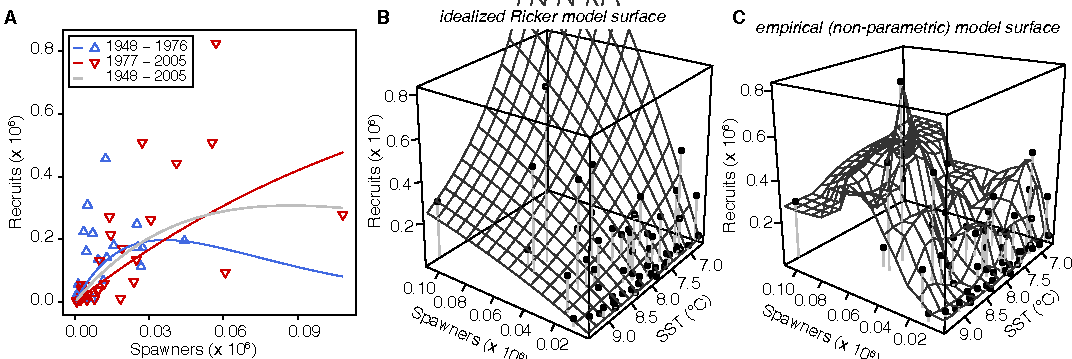
\includegraphics[width=\maxwidth{\textwidth}]{fig_salmon_1.pdf}\end{center}
\caption[Model output for the Ricker, extended Ricker, and multivariate EDM models.]{\textbf{Model output for the Ricker, extended Ricker, and multivariate EDM models.}\newline
(A) Ricker curves for the Seymour stock of Fraser River sockeye salmon are quite different for the early (blue; 1948--1976 brood years) vs. later (red; 1977--2005) time segments (triangles are observed data). Even fit to the whole time series (gray line), large errors remain. (B and C) Model output (surfaces; points are observed data) from the extended Ricker model (B) and EDM (C) using spawner abundance and Pine Island April SST to forecast recruitment of Seymour sockeye salmon. Although the Ricker model varies smoothly, it can forecast recruitment to be many times higher than the historical maximum. In the EDM model, however, the relationship between temperature and spawners is defined empirically by the data and, thus, more realistically depicted.}
\label{fig_salmon_model_surface}
\end{figure}

A common problem when applying the parametric approach to nonlinear systems is that of ephemeral fitting. That is, although population models may assume that demographic parameters such as growth rate or carrying capacity are fixed constants; these quantities are often observed to vary in time or in relation to other variables (e.g., resource availability, changing climate regimes) when tested on actual data \cite{Walters_1987}. This principle is illustrated in Figure \ref{fig_salmon_model_surface}A, where the Ricker spawner-recruit relationship is fit to the early (1948-1976) and late (1977-2005) halves of the time series from the Seymour stock. Very different relationships emerge in these two time periods, conflicting with the assumption of a fixed equilibrium and constant parameter values. Indeed, Beamish et al. \cite{Beamish_2004} found that the Ricker model fit better when constrained by climate regimes, suggesting that the spawner-recruit relationship does vary in time, a fact consistent with the general notion of nonlinear state dependence \cite{Sugihara_2012, Deyle_2013}.

At its core, nonlinear dynamics (which are known to be ubiquitous in marine species \cite{Hsieh_2005, Glaser_2014a}) occur when variables have interdependent effects; this can be problematic when applying a reductionist approach to understand nonlinear systems. For example, in laboratory experiments, guppies (\emph{Poecilia reticulatus}) preferentially eat Drosophila or tubificid worms depending on which prey is more abundant \cite{Murdoch_1975}. Thus, the strength of predation on, say, Drosophila, will change depending on the abundance of tubificid worms. This prey switching behavior typifies nonlinear state-dependence, whereby different components cannot be treated independently, as would be the case in a linear system or even a nonlinear system approximated at equilibrium. Consequently, applying a model that assumes separability of effects (e.g., vector autoregression \cite{Engle_1987}) to a system that is actually nonlinear can give the appearance of nonstationarity or stochasticity even when the underlying mechanisms are unchanged and deterministic.

Nonlinearity is also known to affect the correct identification of causal drivers--a key prerequisite for understanding and predicting system behavior.  In nonlinear systems, because interacting variables can exhibit transient (mirage) correlations that change in magnitude or sign \cite{Sugihara_2012, Deyle_2013}, the use of correlation to identify causal environmental variables can be misleading, producing both false positives (i.e., correlation does not imply causation) and false negatives (i.e., lack of correlation does not imply a lack of causation). Given the prevalence of nonlinear interactions in ecology, mirage correlations can be misleading. Indeed, a meta-analysis examining the robustness of correlations between recruitment and the environment \cite{Myers_1998} found that only 28 out of 74 initially significant correlations were upheld when subsequent data were included.

Even when causal variables are known, their inclusion into improperly formulated models can produce conflicting results. For example, with sockeye salmon in the Fraser River: although anomalous oceanic conditions experienced by juveniles are thought to be responsible for the low abundance of returning adults in 2009 \cite{Peterman_2011, Cohen_2012, Thomson_2012}, extensions of the standard Ricker model that explicitly include environmental factors surprisingly show no significant improvements in the actual forecasts \cite{Grant_2010, MacDonald_2012, Grant_2013}. A simple explanation for this apparent contradiction is that the extended Ricker model does not accurately portray the relevant interaction between the oceanic environment and sockeye salmon. Indeed, the model naively assumes that the environment acts on recruitment dynamics independently with a constant multiplicative effect (e.g., a 1$^\circ$C decrease in temperature always doubles recruitment regardless of other factors important to the state of the system). While temperature, in all likelihood, does affect recruitment, it probably does not follow this arbitrary form. We demonstrate this by fitting the model to Pine Island sea surface temperature (SST) and Seymour spawner-recruit data (Figure \ref{fig_salmon_model_surface}B), finding that the model predicts unrealistically high recruitment (much higher than the historically observed maximum) for hypothetical (but plausible) conditions of high spawner abundance and low temperature. Thus, although the equation may appear reasonable as a hypothesis, it apparently does not  incorporate the environment realistically.

\subsection{Empirical Dynamic Modeling}
In contrast to fitting an assumed set of equations, Empirical Dynamic Modeling (EDM) instead relies on time series data to reveal the dynamic relationships among variables as they occur \cite{Dixon_1999, Sugihara_2012, Sugihara_1990, Liu_2012, Glaser_2014}. By extracting these relationships empirically, EDM accommodates potentially complex and changing interactions that cannot be described in a simple set of equations. Thus, prediction accuracy with EDM is constrained by the quantity and quality of data rather than by the hypotheses represented in a set of equations (which may be subject to process error due to false or incomplete specification \cite{Sugihara_1994}).

Fundamental to EDM is the concept of a time series as an observation on a dynamic system. Broadly speaking, a dynamic system can be viewed as a set of states (d-dimensional vectors where each coordinate is a system variable) and deterministic rules (governing dynamics) for how the states evolve over time. Collectively, the set of states and their trajectories forms an ``attractor manifold'', and projecting the motion on this manifold to a coordinate axis produces a time series of the corresponding variable (Figure \ref{fig_salmon_lorenz_reconstruction}A). For example, in a simple predator-prey system where the system evolves as a function of the two abundances, the system state could be represented as the ordered pair of predator and prey abundances. This system state can be projected onto the prey coordinate axis to produce a time series of prey abundance, though many other observation functions are also possible (e.g., predator abundance, average number of prey for each predator).

In theory, with time series for all the system variables, it would be possible to reconstruct the original attractor manifold by plotting each time series as a separate coordinate. In practice, however, we typically do not have these data or know the identity of all relevant variables. Fortunately, a fundamental mathematical result proves that information about the entire system is contained in any one variable \cite{Takens_1981, Deyle_2011}, meaning that a shadow version of the original attractor can be constructed from just a single time series. This is accomplished by substituting lags of that time series for the unknown or unobserved variables (Figure \ref{fig_salmon_lorenz_reconstruction}B). These essential mechanics of EDM are detailed in \cite{Sugihara_2012} and crisply summarized in a short animation (SI Movie).

Although a single time series is usually sufficient to reconstruct a system's dynamics, there are exceptions (e.g., it is not a closed system). In the case of sockeye salmon, abundance alone may not skillfully predict future returns because they are influenced by external environmental factors. Here, the environment may be thought to act as stochastic external forcing, necessitating its inclusion as an additional coordinate in a multivariate reconstruction \cite{Dixon_1999, Deyle_2013, Deyle_2011}. We demonstrate this by using spawners and sea-surface temperature to predict recruitment (Figure \ref{fig_salmon_model_surface}C). Unlike a parametric model in which a hypothesized interaction must be specified in advance (the extended Ricker model, Figure \ref{fig_salmon_model_surface}B), the empirical surface in Figure \ref{fig_salmon_model_surface}C makes no assumptions about the relationship between variables, but instead captures the interaction between density-dependence and environmental conditions as revealed by the data: ocean temperatures have a stronger effect on recruitment when spawner abundance is low. 

\subsection{Fraser River Sockeye Salmon}

\begin{figure}[!ht]
\begin{center}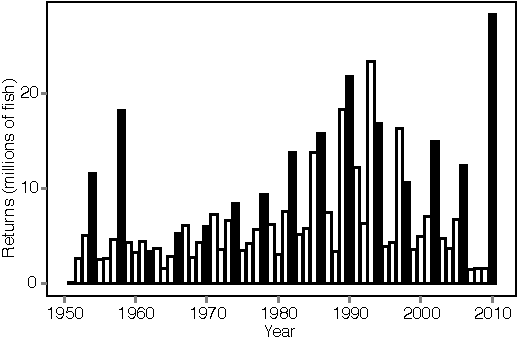
\includegraphics[width=\maxwidth{\textwidth}]{fig_salmon_2.pdf}\end{center}
\caption[Combined returns of Fraser River sockeye salmon.]{\textbf{Combined returns of Fraser River sockeye salmon.}\newline
Total returns (Dataset S1) for Fraser River sockeye salmon combined across stocks (1954 cycle line in black). Although not all stocks exhibit cyclic dominance, and those that do are not synchronized, cycles are still visible in the aggregated returns.}
\label{fig_salmon_returns}
\end{figure}

\begin{figure}[!ht]
\begin{center}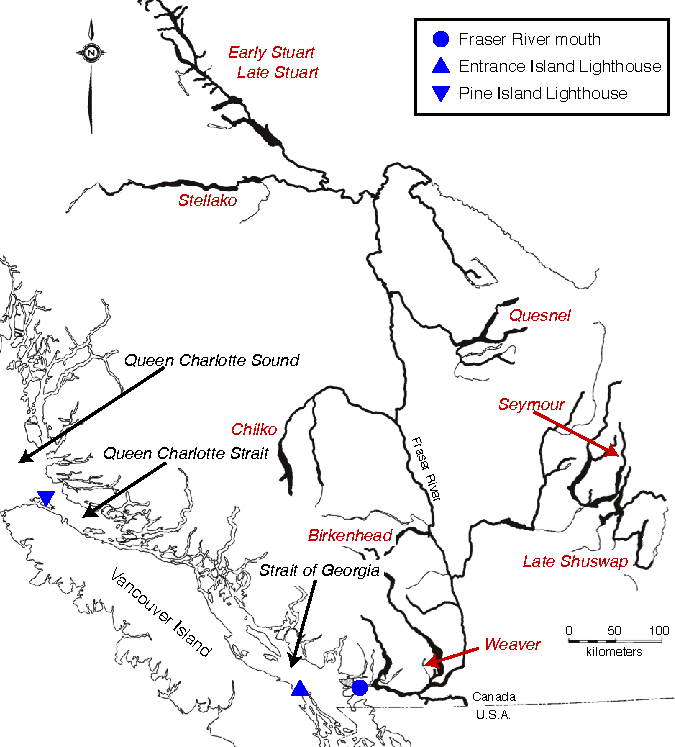
\includegraphics[width=\maxwidth{\textwidth}]{fig_salmon_3.pdf}\end{center}
\caption[Early ocean environment for Fraser River sockeye salmon.]{\textbf{Early ocean environment for Fraser River sockeye salmon.}\newline
Upon exiting the Fraser River, juvenile sockeye salmon migrate north through the Strait of Georgia, spending up to a month moving through this ecosystem \cite{Preikshot_2012}, before continuing through Queen Charlotte Strait and into Queen Charlotte Sound. Red labels for the nine stocks studied in this work are located at the approximate spawning sites. Blue triangles denote the locations of the two lighthouses where SST is recorded. Image courtesy of DFO.}
\label{fig_salmon_map}
\end{figure}

In this work, we perform a real-world test comparing EDM and the standard parametric paradigm, by forecasting returns for the 9 most historically abundant stocks of sockeye salmon from the Fraser River system in British Columbia, Canada (Figure \ref{fig_salmon_returns}), of significance to Canada's iconic fisheries. Total returns in this system are highly variable and can span over an order of magnitude: a record low of 1.6 million in 2009 was followed by a record high of 28.3 million in 2010 (Figure \ref{fig_salmon_map}). Although some of this variability occurs because of cyclic dominance \cite{Ricker_1950, Cass_1994}, large interannual fluctuations in mortality and productivity (recruits-per-spawner) are difficult to predict, leading to considerable uncertainties in current parametric forecast models \cite{Grant_2011}. This is suggestive of nonlinear dynamics in this fishery, and indeed, a Canadian federal inquiry \cite{Cohen_2012, Thomson_2012} concluded that recent declines in productivity could not be attributed to any single mechanism, but were likely caused by the interaction of multiple stressors (e.g., predators, food availability, environment). Applying a simple S-map test (p = 0.002) (\nameref{salmon_supplement}, Figure \ref{fig_salmon_nonlinearity}), we confirm the presence of nonlinear dynamics among returns of Fraser River sockeye salmon.

Thus, we apply EDM methods to unravel the mechanisms by which the environment may affect sockeye salmon recruitment. First, we compare the classical Ricker spawner-recruit model with equivalent EDM spawner-recruit models. With nearly all adults returning as age 4 or age 5 fish, we can consider the total returns in a single calendar year to be composed of age 4 and age 5 recruits from different spawning broods. Following \cite{Grant_2010}, we predict annual returns by first estimating total recruitment for each spawning brood year. This recruitment is then partitioned by age, and the age 4 and age 5 estimates from separate brood years combined appropriately to forecast returns (\nameref{salmon_materials}). Note that the time series of spawning abundance and recruitment already account for the effects of the fishery (this information is contained within the time series, see \nameref{salmon_materials}), which enables us to focus on just the natural population dynamics.

Second, to investigate the causal influence of the oceanic environment, we consider forecasts produced by the extended Ricker model and equivalent multivariate EDM formulations. In both cases, if the inclusion of environmental variables significantly improves forecasts (\nameref{salmon_materials}), those variables are taken to have a causal influence on salmon recruitment.

Lastly, to avoid arbitrary fitting and to obtain a robust measure of forecast skill, we apply a 4-fold cross-validation scheme for each model: the model is fit to $\frac{3}{4}$ of the data to predict the remaining $\frac{1}{4}$ out-of-sample, and the procedure is repeated for each $\frac{1}{4}$ segment of the time series.

\begin{figure}[!ht]
\begin{center}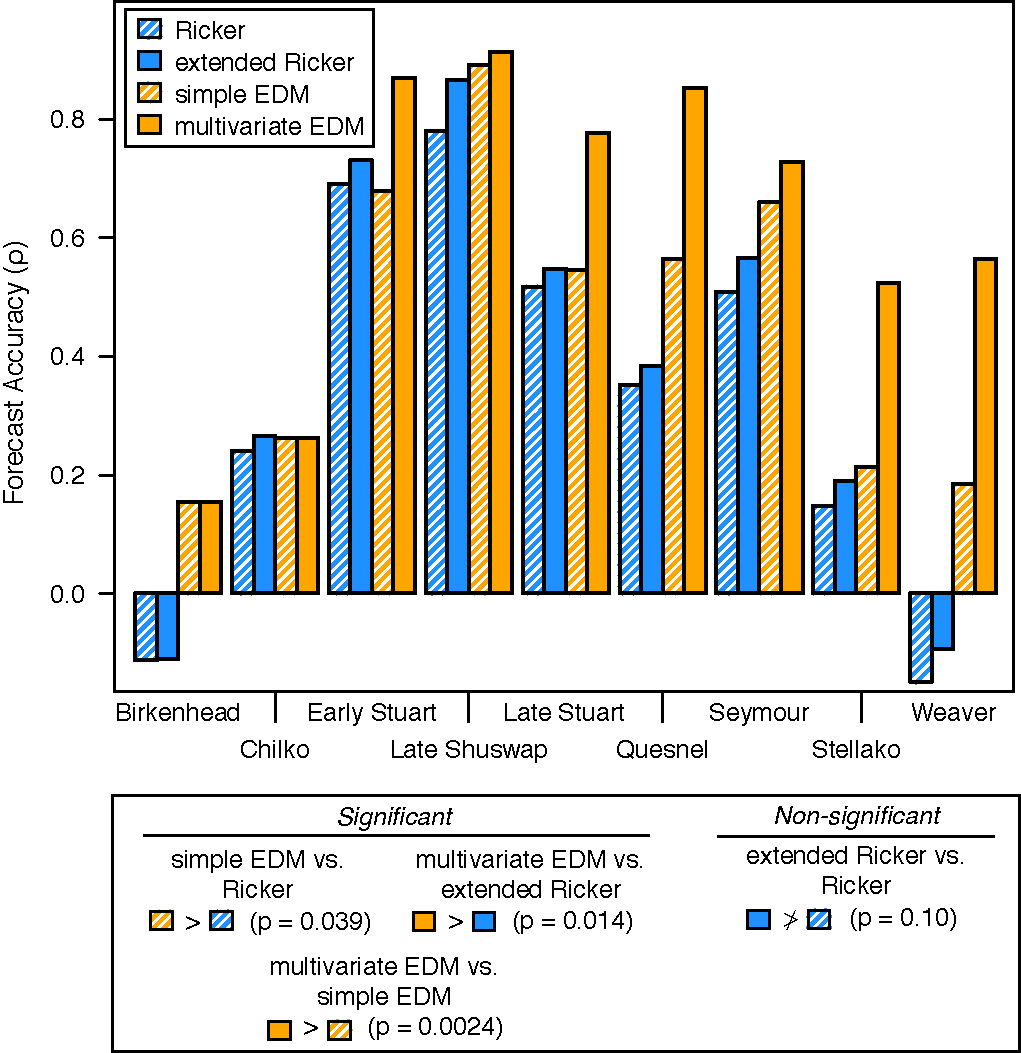
\includegraphics[width=\maxwidth{\textwidth}]{fig_salmon_4.pdf}\end{center}
\caption[Comparison of forecast accuracy.]{\textbf{Comparison of forecast accuracy.}\newline
Comparisons between equivalent EDM and Ricker models show better forecast accuracy for the EDM models [simple EDM vs. Ricker, $t_{(492)} = 1.77$, $P = 0.039$; multivariate EDM vs. extended Ricker, $t_{(492)} = 2.20$, $P = 0.014$]. Additionally, including environmental data significantly improves accuracy for EDM [$t_{(492)} = 2.83$, $P = 0.0024$], but not for the Ricker models [$t_{(492)} = 1.26$, $P = 0.10$].}
\label{fig_salmon_model_comparison}
\end{figure}

\section{Results}

\subsection{Comparison of Spawner-Recruit Forecast Models}

As a fair comparison with the standard Ricker model where spawner abundance is used to predict recruitment, we examine an equivalent EDM spawner-recruit model, but which actually has fewer fitted parameters (\nameref{salmon_materials}). Figure \ref{fig_salmon_model_comparison} shows that this simple EDM model has significantly higher accuracy ($\rho$, correlation between observations and predictions) than the Ricker model, with more accurate forecasts in 8 of 9 cases and significantly lower error overall [mean absolute error (MAE); Figure \ref{fig_salmon_model_comparison_mae}). Nonetheless, predictions for several stocks (Birkenhead, Chilko, Stellako, and Weaver) are not very skillful ($\rho < 0.3$), suggesting that in these cases, there is no simple spawner-recruit relationship (parametric or otherwise). Instead, environmental factors (e.g., sea-surface temperature, food availability) may dominate, and better performance can be obtained by accounting for these external drivers.

\subsection{Incorporating Environmental Influences}

\begin{table}
\caption[Forecast skill of models incorporating the environment]{\textbf{Forecast skill of models incorporating the environment}\newline
D, Fraser River discharge; ET, Entrance Island SST; PDO, Pacific Decadal Oscillation; PT, Pine Island SST.} \label{tab_salmon_forecast_skill}

\begin{center}
\begin{tabular}{lclcrr}
\hline
Stock & Model & Predictors & No. predictions & \multicolumn{1}{c}{$\rho$} &  \multicolumn{1}{c}{MAE} \\
\hline
Birkenhead & Ricker & $S$, $\mathrm{ET}_{\mathrm{jun}}$ & 57 & -0.111 & 0.251 \\
& EDM & $S$ & 57 & 0.156 & 0.259 \\
Chilko & Ricker & $S$, $\mathrm{ET}_{\mathrm{may}}$ & 57 & 0.268 & 0.825 \\
& EDM & $S$ & 57 & 0.264 & 0.839 \\
Early Stuart & Ricker & $S$, $\mathrm{ET}_{\mathrm{apr}}$ & 57 & 0.737 & 0.172 \\
& EDM & $S$, $\mathrm{D}_{\mathrm{apr}}$, $\mathrm{D}_{\mathrm{jun}}$ & 57 & 0.878 & 0.140 \\
Late Shuswap & Ricker & $S$, $\mathrm{ET}_{\mathrm{jun}}$ & 57 & 0.875 & 0.842 \\
& EDM & $S$, $\mathrm{D}_{\mathrm{may}}$, $\mathrm{PT}_{\mathrm{jul}}$ & 57 & 0.923 & 0.821 \\
Late Stuart & Ricker & $S$, $\mathrm{D}_{\mathrm{jun}}$ & 56 & 0.552 & 0.423 \\
& EDM & $S$, $\mathrm{D}_{\mathrm{jun}}$, $\mathrm{ET}_{\mathrm{apr}}$ & 56 & 0.783 & 0.250 \\
Quesnel & Ricker & $S$, $\mathrm{ET}_{\mathrm{jun}}$ & 57 & 0.387 & 2.057 \\
& EDM & $S$, $\mathrm{PT}_{\mathrm{may}}$, $\mathrm{PDO}$ & 57 & 0.861 & 0.729 \\
Seymour & Ricker & $S$, $\mathrm{PT}_{\mathrm{apr}}$ & 57 & 0.571 & 0.076 \\
& EDM & $S$, $\mathrm{PT}_{\mathrm{jul}}$ & 57 & 0.734 & 0.065 \\
Stellako & Ricker & $S$, $\mathrm{ET}_{\mathrm{may}}$ & 57 & 0.191 & 0.250 \\
& EDM & $S$, $\mathrm{PT}_{\mathrm{apr}}$, $\mathrm{PDO}$ & 57 & 0.531 & 0.217 \\
Weaver & Ricker & $S$, $\mathrm{PDO}$ & 39 & -0.094 & 0.215 \\
& EDM & $S$, $\mathrm{D}_{\mathrm{apr}}$, $\mathrm{D}_{\mathrm{may}}$ & 39 & 0.573 & 0.176 \\
\hline
\end{tabular}
\end{center}
\end{table}

As in the actual forecast models \cite{Grant_2010}, we further consider 3 environmental variables (the Pacific Decadal Oscillation (PDO), sea-surface temperature (SST), and Fraser River discharge) observed at different times and locations (12 time series in total). Each of these factors is believed to have a potential effect on recruitment, though significance has yet to be demonstrated in practice. For each stock, we compare the relative performance of the extended Ricker and corresponding multivariate EDM models that incorporate these environmental variables (Table \ref{tab_salmon_forecast_skill}; \nameref{salmon_materials}). Figure \ref{fig_salmon_model_comparison} shows that multivariate EDM is consistently and significantly better at forecasting than the extended Ricker model for all 9 stocks, and is true for both accuracy and precision metrics (Figure \ref{fig_salmon_model_comparison_mae}). Here, the relevant causal influence of these environmental variables is verified by the fact that multivariate EDM models that include them perform significantly better than their simple EDM spawner-recruit counterparts.

By contrast, the extended Ricker models show no significant improvement over the simple Ricker models in any of the stocks. The difference between EDM and Ricker is especially visible for Late Stuart, Quesnel, Stellako, and Weaver, indicating that these particular environmental factors (currently considered in assessments) can explain much of the variability in these stocks, provided they are incorporated reasonably (i.e., with the minimal assumptions of EDM). For Birkenhead and Chilko however, multivariate EDM models performed no better than the simplified stock-recruit versions, hinting that variables other than these are required to understand the dynamics of those stocks.

\section{Discussion}

\subsection{Nonlinearity of Fraser River Sockeye Salmon}

Similar to many marine species \cite{Hsieh_2005, Glaser_2014a}, Fraser River sockeye salmon show strong evidence for nonlinear dynamics (Figure \ref{fig_salmon_nonlinearity}, Table \ref{tab_salmon_nonlinearity}). Thus, it should not be surprising that a simple EDM model, which accommodates nonlinearity, would outperform the assumed spawner-recruit equation of the Ricker model. Furthermore, because sockeye salmon are exposed to different sources of environmentally driven mortality and because it is likely that they integrate these effects in a nonlinear fashion, it should not be surprising that multivariate EDM models that explicitly accommodate relevant environmental factors would show dramatically improved performance. In contrast, the extended Ricker model cannot resolve the nonlinear effect of the environment, and shows only non-significant improvements (that might be expected from having additional degrees of freedom).

\subsection{Identifying Environmental Drivers}

It is believed that growth during the early marine stage for Pacific salmon is a critical period that determines subsequent mortality and recruitment \cite{Beamish_2001, Beamish_2004a}. Thus, it is reasonable to expect that including related environmental variables into models should improve predictions. However, the extended Ricker model did not improve when river discharge, SST, or the PDO (Figure \ref{fig_salmon_model_comparison}, Figure \ref{fig_salmon_model_comparison_mae}) were included. Rather than suggesting that these variables have no effect, it is more likely that the extended Ricker model is incorrectly specified. This is borne out by the fact that these factors produce improved forecasts for many stocks when included non-parametrically in EDM (Figure \ref{fig_salmon_model_comparison}, Figure \ref{fig_salmon_model_comparison_mae}). Thus, our analysis suggests that the tested variables are indeed informative about the relevant environmental conditions experienced by juvenile sockeye salmon. For example, river discharge and SST may indicate primary productivity in the Strait of Georgia and other areas through which juveniles migrate (Figure \ref{fig_salmon_returns}) \cite{Thomson_2012, Beamish_1994, Preikshot_2012}, and the associations between large-scale oceanic climate indicators such as the PDO and Pacific salmon productivity are well-known from other studies \cite{Mantua_1997, Beamish_1997}. While these variables do not reflect direct causal mechanisms, they may be useful as simple indicators of processes that influence salmon survival, thereby improving forecasts when included in the EDM approach.

While individual stocks appear to be sensitive to different environmental factors (Table \ref{tab_salmon_forecast_skill}), we did observe some general patterns: for example, 2 of the 9 stocks (Stellako and Quesnel) identified the PDO as an informative variable (the first-ranked EDM models for these stocks include the PDO as a coordinate), yet the predictability for these stocks is further improved when other variables (river discharge or SST) are included in addition to the PDO. This suggests that the PDO is an incomplete observation on the relevant environment for sockeye, and that local-scale measures of the environment can enhance the information in the PDO index (an ocean basin-scale indicator) (see \nameref{salmon_supplement} for details).

Although our models confirm a general influence of the environment on sockeye salmon recruitment, some stocks appear to be skillfully predicted using only spawner abundance. One explanation for this is that the stocks experience unique environments: they are exposed to different freshwater conditions in their respective nursery lakes, and they exhibit different timings and migration routes as they travel through the Fraser River (T. Whitehouse, DFO, pers. comm.), the Strait of Georgia \cite{Beacham_2014}, and along the west coast of North America \cite{Tucker_2009}. Even with shared environmental influences (e.g., food availability in the Strait of Georgia), nonlinear state-dependence can produce dynamics unique to each stock. Consequently, if these myriad effects are strongly density-dependent, recruitment could be successfully predicted using just spawner abundance. However, if these effects are stochastic (i.e., environmentally-driven), then it will be necessary to include informative indicator variables to improve forecasts.

Apart from multivariate models, an alternative approach to determine causal environmental variables would be to apply the method of convergent cross mapping (CCM, \cite{Sugihara_2012}). However, due to data limitations (in particular, the absence of annual monitoring of each cycle line including the oceanic phase), CCM may not be sufficiently sensitive to resolve causality here (see \nameref{salmon_supplement} for details)

\subsection{Nonuniqueness of Models}

We note that, for a given stock, different EDM models can show similar performance (Table \ref{tab_salmon_multivariate_full}). Although somewhat counter-intuitive, this phenomenon is expected, because the tested variables (river discharge, SST, the PDO) are proxy indicators of the environment. Thus, they may contain redundant information such that different variable combinations are equally informative even as they represent alternative perspectives on the system. This reflects a fundamental property of EDM in that forecast performance depends solely on the information content of the data rather than on how well assumed equations match reality.

To clarify the concept of non-uniqueness, consider the canonical Lorenz attractor (Figure \ref{fig_salmon_lorenz_reconstruction}A). The behavior of this system is governed by three differential equations (Equation \ref{eqn_lorenz}). However, the axes can be rotated to produce 3 new coordinates, $x^\prime$, $y^\prime$, and $z^\prime$ and the equations rewritten in terms of these new coordinates, allowing the system to be described using either representation ($x$, $y$, and $z$ OR $x^\prime$, $y^\prime$, and $z^\prime$) as well as mixed combinations (e.g., $x$, $y$, and $z^\prime$). Thus, with an infinite number of ways to rotate the system, there are an unlimited number of ``true variables'' and ``true models.'' In the case of sockeye salmon, the similar performance of different models (Table \ref{tab_salmon_multivariate_full}) does not mean that one or the other model is incorrect; instead, it reflects the fact that the environmental variables are indicators of the same general mechanism, and so different variable combinations can be equally informative for forecasting recruitment.

Again, we emphasize that including a variable does not imply a direct causal link -- variables in an EDM model improve forecasts because they are informative; it does not mean that the included variables are proximate causes. Importantly, the converse does not hold either: a variable could be causal and yet not appear in the multivariate EDM; this might occur when multiple stochastic drivers affect recruitment in an interdependent way, necessitating that a model include measurements of all the drivers to account for their combined effect. For example, although none of the tested variables seem to improve forecasts for the Birkenhead stock (Table \ref{tab_salmon_multivariate_full}), this does not mean that these sockeye salmon are insensitive to SST, river discharge, and the PDO. Rather, it suggests that the effect of these variables may be modulated by other factors not considered here.

\subsection{Data Requirements of EDM}

Using EDM is fundamentally a data-driven approach: thus, it is important to ensure that time series are of sufficient length to recover dynamics. For example, Sugihara et al. \cite{Sugihara_2012} suggest that at least 35-40 points might be necessary as a rough minimum, though methods exist for using dynamically similar replicates in cases where time series are shorter \cite{Hsieh_2008}. For many systems, however, the data requirements of EDM mean that increased budgets and additional sampling effort will be important to support long-term continuous observations and generate sufficient time series. We note, though, that it is not necessary to sample all putatively relevant drivers, because different measurements are often substitutable as proxies for true proximal causes.

When data requirements are met, however, we note that collecting additional data can further improve accuracy and precision of EDM models. Consider the simplex projection method, which uses nearest-neighbor analogues to approximate system behavior. With each new data point, more analogues are available (the reconstructed manifold becomes denser), and so these approximations become more precise. Thus, EDM models will improve with longer time series. In contrast, a parametric model will benefit from more data only when the assumed equations are essentially correct. In the case of the classic Ricker model in Figure \ref{fig_salmon_model_surface}A, it is clear that similar levels of spawner abundance yield very different levels of recruitment, and so any simple function relating the two cannot fully explain the scattered observations. Adding more data may result in more ``precise'' parameter estimates, but individual errors will remain large when the underlying process is more complex than the assumed model can portray.

\subsection{Alternative Parametric Models}

In this work, we use the classical and extended Ricker models as examples of the parametric approach, but acknowledge that there are alternative models considered by the DFO for Fraser River sockeye salmon \cite{Peterman_2000, Haeseker_2007, Haeseker_2008, Grant_2012}. While some of these models may fit the data better, this does not always reflect a model's true performance in out-of-sample forecasting. For example, a modified Ricker model that allows parameters to randomly drift over time \cite{Peterman_2000} will explain variations in the data better than the static alternative, because doing so can indirectly track nonlinear state-dependence. However, instead of a mechanism for why parameters change, such models based on the Kalman filter \cite{Kalman_1960} typically use forward information (i.e., observations at time $t+1$ help to estimate the growth rate at time $t$), and thus do not actually ``predict.'' Consequently the actual forecast performance of such models will be overestimated by their fit to historical data. A more fundamental concern with the parametric approach is that it requires explicit equations to model the effects of included variables. Such equations may be overly simplified (e.g., linear correlations) and unable to accommodate the state-dependent effects that occur in nonlinear systems.

\subsection{Final Remarks}

EDM addresses two important challenges for modeling natural systems. First, EDM identifies relevant variables and interactions empirically and dynamically \cite{Sugihara_2012}; this is in contrast to the conventional approach where the use of parametric equations poses the dual risks of model misspecification \cite{Sugihara_1994} as well as variable misidentification \cite{Sugihara_2012, Deyle_2013, Myers_1998}. Importantly, EDM allows proxy variables to be used, which can be a boon when observations on key processes (e.g., mortality) are lacking but indirect measurements (e.g., SST) are available. Second, the equation-free approach of EDM produces more accurate forecasts than equivalent parametric models using the same data. As Perretti et al. \cite{Perretti_2013} have shown, even when a correct parametric model is known, fitting parametric models can be problematic, and is an important concern with many systems exhibiting nonlinear behavior \cite{Hsieh_2005, Glaser_2014a}. In contrast, EDM models can capture dynamic information and explain behavior that may be misclassified as random by parametric fitting procedures.

Consequently, the dynamic perspective of EDM has much to offer for modeling nonlinear systems, representing a viable framework (with minimal assumptions) for system identification and robust forecasting. When parametric models are required, EDM can also be used in a complementary role to identify causal links, recover variable relationships, and even guide the construction of reliable equation-based models \cite{Crutchfield_1987}. This represents a practical way to perform data-driven modeling instead of starting with complex parametric models (end-to-end ecosystem models, such as Ecopath with Ecosim \cite{Christensen_2004}), which often make strong assumptions and require large amounts of data to parameterize.

Moreover, EDM models can also serve as direct substitutes for their parametric equivalents. Here, our simple and multivariate EDM models are formulated similarly to their Ricker-based counterparts: using spawner abundance (and the environment) to forecast returns. Some simple extensions to the methods, such as the development of uncertainty estimates (see \nameref{salmon_supplement}, Figure \ref{fig_salmon_standard_error}), will enable these models to be integrated into the current management framework that uses parametric models. Thus, we believe that EDM has great potential as a tool for understanding and forecasting nonlinear ecosystems: by operating without assumed equations, it can be beneficial when exact mathematical descriptions are not available.

\section{Materials and Methods}
\label{salmon_materials}

\subsection{Data}

We analyze yearly time series data for the 9 historically most abundant stocks (Birkenhead, Chilko, Early Stuart, Late Shuswap, Late Stuart, Quesnel, Seymour, Stellako, and Weaver) of sockeye salmon from the Fraser River system. Data span brood years 1948--2005, except for Late Stuart and Weaver, where data begin in 1949 and 1966, respectively. We consider only single-stock models, so notation and equations are given as for a single stock.

$S_t$ is the number of effective female spawners in brood year $t$, and $R_t$ is the corresponding recruitment (returning adults). Recruitment is partitioned by age: $R_{a, t}$  is the number spawned in year $t$ and returning at age $a$ in year $t + a$. Following \cite{Grant_2010}, total recruitment is the sum of age 4 and age 5 recruits: $R_t = R_{4, t} + R_{5, t}$. In contrast, total returns, $N_y$, are the adults that return to spawn in calendar year $y$, and computed as $N_y = R_{4, y-4} + R_{5, y-5}$. As explained below, recruitment is forecast from spawner abundance, and age 4 and age 5 recruits (from different brood years) are summed to estimate total returns in a given calendar year. Note that both recruitment and returns are computed as catch + escapement + en-route loss, while spawner abundance is based on observations of escapement and egg production \cite{Grant_2011}. Thus, both spawner abundance and recruitment account for the effects of catch, and the models we consider here focus just on the population dynamics of this system.

We investigate 3 environmental variables: the Pacific Decadal Oscillation (PDO), sea-surface temperature (SST), and Fraser River discharge. For the PDO, one annual time series is constructed as the average of monthly values from November to March \cite{Mantua_1997}. SST measures are monthly averages from two lighthouse stations (Entrance Island: April to June and Pine Island: April to July). River discharge is measured at Hope; we include peak daily flow and monthly averages (April to June). Fraser River sockeye salmon enter the ocean at age 2, so the environmental data are lagged 2 years to line up with ocean entry time.

\subsection{Attractor Reconstruction}

The goal of attractor reconstruction is to approximate the originating dynamic system using time series data. The simplest construction uses successive lags of a single time series \cite{Takens_1981, Packard_1980}: given time series $\{x_t\}$, $E$-dimensional vectors $\vec{x}_t$ are composed of $E$ lags of $x$, each separated by a time step $\tau$: $\vec{x}_t = \langle x_t, x_{t-\tau}, \dots x_{t-(E-1)\tau}\rangle$.

Generalizations of Takens' theorem \cite{Deyle_2011, Sauer_1991} permit attractor reconstructions using multiple time series. For example, with $\{x_t\}$ and $\{y_t\}$ observed from the same system, one possible reconstruction forms vectors as $\langle x_t, y_t, y_{t-\tau}\rangle$. To account for different scaling between variables, each time series is first linearly transformed to have mean $= 0$ and variance $= 1$.

\subsection{Simplex Projection and S-map}

Simplex projection estimates the trajectory (i.e., forecasts) of a novel system state by computing a weighted average of the trajectories of that state's nearest neighbors \cite{Sugihara_1990}. Given an attractor reconstruction, and a novel state $\vec{x}_s$, we first find the $b$ nearest neighbors (typically setting $b = E + 1$) that are closest to $\vec{x}_s$: these neighbors are the vectors $\vec{x}_{n(s, i)}$ where $n(s, i)$ designates the time index of the $i$th closest neighbor to $\vec{x}_s$. So, $\vec{x}_{n(s, 1)}$ is the closest neighbor to $\vec{x}_s$, $\vec{x}_{n(s, 2)}$ is the second closest neighbor, etc. We then evolve the neighbors forward, and compute a weighted average of the forward evolutions ($h$ time steps into the future) to estimate $\vec{x}_{s+h}$:

\begin{equation}
\label{eqn_simplex}
\hat{\vec{x}}_{s+h}=\left(\sum_{i=1}^{b}{w_i\left(s\right)\vec{x}_{n(s, i)+h}}\right) \bigg/ \sum_{i=1}^{b}{w_i\left(s\right)}.
\end{equation}

The weights, $w_i(s)$, are based on the distance between $\vec{x}_s$ and its $i$th neighbor, $\vec{x}_{n(s, i)}$, scaled to the distance to the nearest neighbor: \\$w_i(s) = exp\left(-d(\vec{x}_s, \vec{x}_{n(s, i)})/d(\vec{x}_s, \vec{x}_{n(s, 1)})\right)$ and $d(\vec{x}_s, \vec{x}_t)$ is the Euclidean distance between the vectors $\vec{x}_s$ and $\vec{x}_t$.

In most cases, we desire forecasts of a scalar value rather than of the full system state. This is possible when the variable to be forecast, $y$, is an observation on the same dynamic system. As such, there will be a correspondence between $\vec{x}_t$ and the scalar value of $y_t$, and we can adjust equation \ref{eqn_simplex} to compute a weighted average of the corresponding values of $y$:

\begin{equation}
\label{eqn_simplex_scalar}
\hat{y}_{s+h} = \left(\sum_{i=1}^{b}{w_i\left(s\right)y_{n(s, i)+h}}\right) \bigg/ \sum_{i=1}^{b}{w_i\left(s\right)}.
\end{equation}

The S-map procedure computes a local linear map between lagged-coordinate vectors and a target variable and is often used to test for nonlinear state-dependence \cite{Sugihara_1994}. It includes a tuning parameter, $\theta$, that controls the weights associated with individual vectors: $\theta = 0$ reduces the S-map to a linear autoregressive model of order $E$, while $\theta > 0$ gives more weight to nearby states when computing the local linear map, thus allowing for nonlinear behavior. Following \cite{Glaser_2014a, Hsieh_2006}, we test for nonlinearity by computing the decrease in forecast error (MAE) as $\theta$ is tuned to be greater than 0 (see \nameref{salmon_supplement} for details).

\subsection{Model Descriptions}

We formulate EDM models to forecast recruitment from spawner abundance, combining age 4 and age 5 recruits (from different brood years) to estimate total returns in a given calendar year. Acknowledging the persistent 4-year quasicycle, the time series of recruits and spawners are scaled so that each cycle line has mean 0 and variance 1: $S^\prime_t = \left(S_t - \mu_k(S)\right)/\sigma_k(S)$ and $R^\prime_t = \left(R_t - \mu_k(R)\right)/\sigma_k(R)$, where $k = 1, 2, 3, \mathrm{or } 4$, depending on cycle line and can be computed as $k = 1 + ((t-1) \bmod 4)$. $\mu_k$ and $\sigma_k$ are the mean and standard deviation, respectively, for the $k$th cycle line.

The simple EDM model approximates the system state with 1 lag of the transformed spawner abundance:
\begin{equation}
\vec{x}_t = \langle S^\prime_t \rangle.
\end{equation}

Forecasts of the age 4 and age 5 recruits, $R^\prime_{4, t}$ and $R^\prime_{5, t}$, are made using simplex projection. Here, the two nearest neighbors of $S^\prime_t$ are identified, and the corresponding values of $R^\prime_{4, t}$ (or $R^\prime_{5, t}$) are combined in a weighted average to produce a forecast. These forecasts are transformed back into raw values, $\hat{R}_{a, t} = \hat{R}^\prime_{a, t} \cdot \sigma_k(R_a) + \mu_k(R_a)$, and age 4 and age 5 recruits are combined to produce a forecast of total returns, $\hat{N}_y = \hat{R}_{4, y-4} + \hat{R}_{5, y-5}$.

The multivariate models combine spawner data with up to 2 environmental indicators:
\begin{align}
\begin{split}
\vec{x}_t &= \langle S^\prime_t, U^\prime_{t+2} \rangle\\
\vec{x}_t &= \langle S^\prime_t, U^\prime_{t+2}, U^{\prime\prime}_{t+2} \rangle,
\end{split}
\end{align}

where $U^\prime_{t+2}$ (or $U^{\prime\prime}_{t+2}$) is one of the environmental time series described previously, normalized to have mean $= 0$ and variance $= 1$. Just as in the simple EDM model, forecasts of the age 4 and age 5 recruits are made using simplex projection and combined to produce a forecast of total returns. However, because including environmental variables increases the embedding dimension, three nearest neighbors are used for models that include one environmental coordinate, and four nearest neighbors for models that include two environmental coordinates.

Following \cite{Grant_2010}, we use the standard Ricker model to estimate total recruitment and then partition it into age 4 and age 5 fish. age 4 and age 5 fish from separate brood years are combined to forecast the number of returns:
\begin{align}
\begin{split}
\hat{R}_t &= S_t \exp{(\alpha - \beta S_t)},\\
\hat{N}_y &= \hat{R}_{y-4} \cdot p_4 + \hat{R}_{y-5} \cdot (1 - p_4),
\end{split}
\end{align}

where $p_4$ is the average fraction of recruits that return as age 4 fish. The extended Ricker model is similar, but includes an additional term in the exponent for an environmental covariate:

\begin{equation}
\hat{R}_t = S_t \exp{(\alpha - \beta S_t + \gamma U_{t+2})}.
\end{equation}

\subsection{Fitting Procedure and Performance Measures}

To avoid testing all combinations of (and overfitting) the environmental variables in the EDM model, we sequentially add the environmental variable that most improves forecast accuracy ($\rho$, the correlation between observed and predicted values). If none of the variables improve forecasts when added, then no further environmental variables are included. Thus the best EDM model for some stocks may have only 0 or 1 environmental variable (Table \ref{tab_salmon_forecast_skill}). Similarly, for the extended Ricker model, we choose the environmental variable that gives the highest $\rho$.

The Ricker models were fit using R 3.0.2 (\url{http://www.r-project.org/}), the Rjags package (\url{http://cran.r-project.org/web/packages/rjags/index.html}), and \linebreak JAGS 3.2.0 (Just Another Gibbs Sampler; \url{http://mcmc-jags.sourceforge.net/}) following the procedure outlined in \cite{Grant_2010}. Medians of the posterior distribution are used to obtain point estimates suitable for comparison. The EDM models were constructed using R 3.0.2 and the rEDM package (\url{https://github.com/ha0ye/rEDM}). The package can be installed with the following lines of R code:
\begin{verbatim}
library(devtools)
install_github("ha0ye/rEDM")
\end{verbatim}
R scripts for the models and data files can be found in the supplementary information.

All forecasts are made using a 4-fold cross-validation procedure. To quantify model performance, we use Pearson's correlation coefficient ($\rho$) between observed and predicted returns as a measure of accuracy and MAE as a measure of error. Comparisons of $\rho$ between models uses a one-sided $t$ test with SE calculated using the HC4 estimator from \cite{Cribari-Neto_2004} and with adjusted degrees of freedom as suggested by \cite{Wilcox_2009}. Improvement in MAE is computed using a one-sided paired $t$ test for the difference, treating each forecast as an independent sample. To compute an aggregate statistic combining all 9 stocks, we first scale the observations and predictions for each stock so that the observed returns have mean $= 0$, variance $= 1$, and then combine the normalized values across stocks. The comparisons of $\rho$ and MAE are done using this combined set of observations and predictions (Figure \ref{fig_salmon_model_comparison}, Figure \ref{fig_salmon_model_comparison_mae}).

\section{Supplementary Information}
\label{salmon_supplement}

\begin{figure}[!ht]
\begin{center}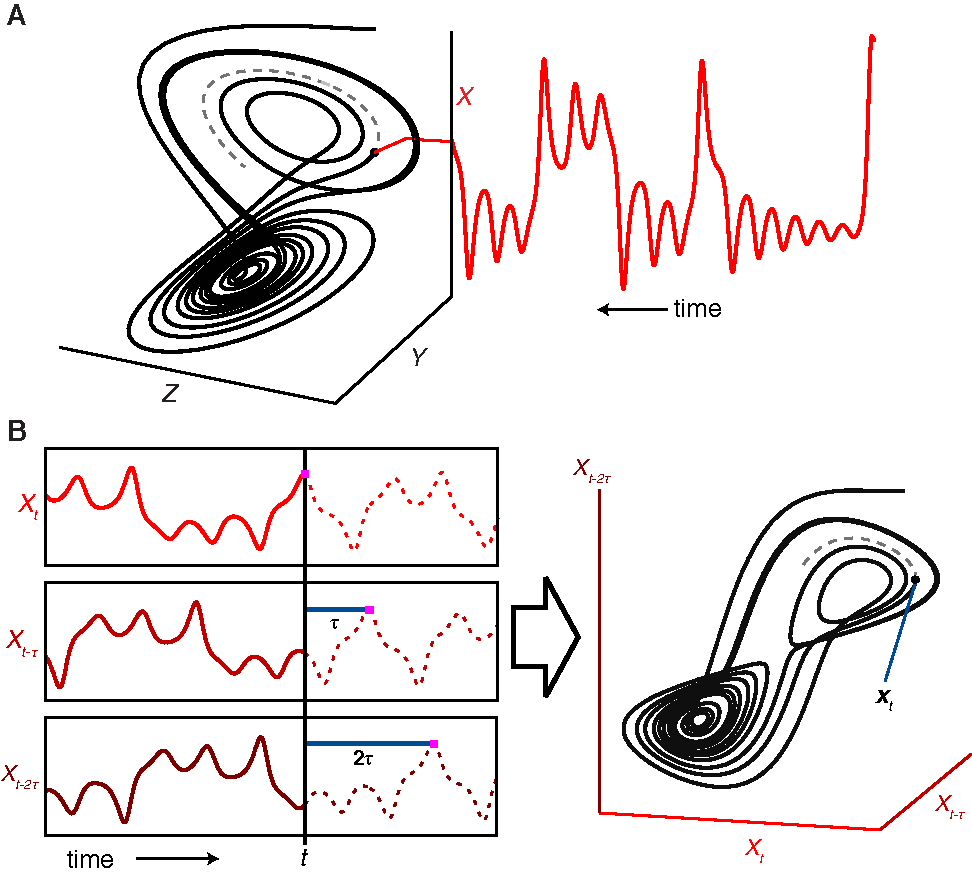
\includegraphics[width=\maxwidth{\textwidth}]{fig_salmon_s1.pdf}\end{center}
\caption[Reconstruction of system dynamics from a time series.]{\textbf{Reconstruction of system dynamics from a time series.}\newline
(A) Projecting the motion of the canonical Lorenz attractor onto the $x$-axis yields a time series for variable $x$. (B) Successive lags (with time step $\tau$) of the time series $x_t$ are plotted as separate coordinates to form a reconstructed ``shadow'' manifold that preserves essential mathematical properties of the original system (and is visually similar).}
\label{fig_salmon_lorenz_reconstruction}
\end{figure}

\subsection{Attractor Reconstruction from Time Series}

Broadly speaking, dynamic systems can be described as a set of states (i.e. a manifold) and rules (governing dynamics or hidden equations) for how the states evolve over time. Motion on the manifold can be projected onto a coordinate axis, forming a time series (Figure \ref{fig_salmon_lorenz_reconstruction}A). More generally, however, any set of sequential observations of the system state (i.e., a function that maps the state onto the real number line) is a time series.

For example, the Lorenz attractor (a simplified description of turbulent flow in the atmosphere \cite{Lorenz_1963}) is a dynamic system where the states are 3-dimensional vectors with coordinates $x$, $y$, and $z$, and whose motion is governed by three differential equations (Equation \ref{eqn_lorenz}).

\begin{align}
\label{eqn_lorenz}
\begin{split}
\frac{dy}{dt} &= 10(y-x)\\
\frac{dy}{dt} &= x(28-z)-y\\
\frac{dz}{dt} &= xy - \frac{8}{3}z
\end{split}
\end{align}

In an ecological setting, these variables could represent the abundances of different species (e.g., salmon, zooplankton, and phytoplankton), with the equations capturing the biological processes of growth, death, and predation. The projection of the system state onto one of the axes gives a time series for the population corresponding to that variable (Figure \ref{fig_salmon_lorenz_reconstruction}A).

If one knew all the relevant variables of a system, their time series could be used to reconstruct the original manifold, by plotting each variable as a separate coordinate. Given time series of sufficient length, it might even be possible to derive the equations of motion for that system. However, in nature, the system may be highly complex (hundreds or thousands of interacting variables or components), and time series are generally short. The method of time-delay embedding \cite{Takens_1981, Crutchfield_1987} offers a solution to this problem; reconstructions of a dynamic system can be made using successive lags of a single time series (Figure \ref{fig_salmon_lorenz_reconstruction}B). Takens' theorem \cite{Takens_1981} states that, if enough lags are taken, this form of reconstruction is generically a diffeomorphism and preserves essential mathematical properties of the original system. In other words, local neighborhoods (and their trajectories) in the reconstruction map to local neighborhoods (and their trajectories) of the original system. This also permits forecasting, by finding nearest neighbors from among the historical record and using their behavior to estimate how the system will evolve through time (e.g., simplex projection, see \nameref{salmon_materials}).

\begin{figure}[!ht]
\begin{center}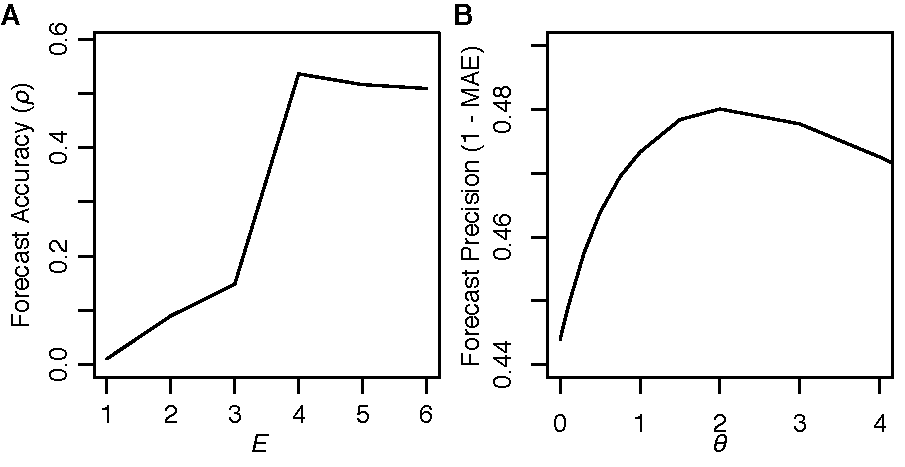
\includegraphics[width=\maxwidth{\textwidth}]{fig_salmon_s2.pdf}\end{center}
\caption[Nonlinearity in Fraser River sockeye salmon.]{\textbf{Nonlinearity in Fraser River sockeye salmon.}\newline
Following \cite{Hsieh_2008}, we concatenate time series of returns for 9 stocks. (A) Forecasting returns using simplex projection, 4 is identified as the optimal embedding dimension. (B) Using the S-map procedure, forecast skill is highest for $\theta \sim 2$ ($P = 0.002$), which demonstrates nonlinear state dependence in salmon dynamics.}
\label{fig_salmon_nonlinearity}
\end{figure}

\begin{table}
\caption[Nonlinearity tests for individual stocks.]{\textbf{Nonlinearity tests for individual stocks.}\newline
$E$ is embedding dimension, $\theta$ is the optimal value of the nonlinear tuning parameter, $\Delta$MAE is the difference in error between the model at the optimal value of $\theta$ and the model at $\theta = 0$ (negative values indicate a decrease in error, or improvement with $\theta > 0$), $P$ value is for a randomization test with 500 iterations (* indicates significance at the $\alpha = 0.10$ level).}
\label{tab_salmon_nonlinearity}

\begin{center}
\begin{tabular}{lrrrrr}
\hline
stock & $E$ & $\theta$ & $\Delta$MAE & $P$ value & significantly nonlinear? \\
\hline
Birkenhead & 5 & 0 & 0 & 0.494 & no \\
Chilko & 6 & 2 & -0.070 & *0.024 & yes \\
Early Stuart & 6 & 4 & -0.023 & *0.050 & yes \\
Late Shuswap & 4 & 2 & -0.389 & *0.014 & yes \\
Late Stuart & 8 & 3 & -0.054 & *0.060 & yes \\
Quesnel & 7 & 4 & -0.298 & *0.008 & yes \\
Seymour & 8 & 0.5 & -0.002 & 0.162 & no \\
Stellako & 7 & 2 & -0.025 & *0.014 & yes \\
Weaver & 1 & 0 & 0 & 0.496 & no \\
\hline
\end{tabular}
\end{center}
\end{table}

\subsection{Identifying nonlinearity in sockeye salmon dynamics}

One application of EDM is to identify nonlinear dynamics in time series. For the Fraser River system, we first consider the 9 stocks in aggregate. Following \cite{Hsieh_2008}, each time series of returns is linearly transformed to have mean $= 0$ and variance $= 1$. This preserves the quasicyclic behavior of each stock, but corrects for the relative magnitude across different stocks. The normalized time series are joined together end-to-end, in effect treating them as 9 instances of a single time series. Using simplex projection with $\tau = 1$ and predicting 1 year into the future, forecast skill ($\rho$) is maximized when 4 successive lags are used (Figure \ref{fig_salmon_nonlinearity}A). This is somewhat expected, because the quasicyclic nature of these returns has a 4-year periodicity: knowing the previous 4 years is sufficient to identify the current phase and estimate the current magnitude of returns.

Next, we employ the S-map procedure \cite{Sugihara_1994}, which compares equivalent linear and nonlinear models (adjusting a tuning parameter, $\theta$) to test for nonlinear dynamics. When $\theta = 0$, all points are weighted equally, and the model reduces to an autoregressive model of order $E$. For $\theta > 0$, nearby points are given stronger weighting, allowing the model to be adaptive to local influences and therefore, nonlinear. If the behavior of sockeye returns is purely periodic, then the linear model should have the highest forecast skill, because it can smooth out errors over the entire data set. However, Figure \ref{fig_salmon_nonlinearity}B shows that forecast skill peaks when $\theta$ is ~ 2, which is evidence for nonlinearity in the aggregate time series. Using the randomization test of \cite{Hsieh_2006, Glaser_2014a}, this improvement in forecast skill (decrease in MAE) is significant with $P = 0.002$.

As noted in \cite{Hsieh_2008}, nonlinearity may appear as an artifact when aggregating linear time series with somewhat different dynamics. Therefore, to confirm the presence of nonlinearity, we also apply the S-map to each stock individually, using the same randomization test for whether the improvement in forecast error (MAE) is significant at the $\alpha = 0.10$ level (Table \ref{tab_salmon_nonlinearity}). Overall, these results are encouraging: we find 6 of the 9 stocks to be significantly nonlinear. We note, however, that the lack of significant nonlinearity in the Birkenhead, Seymour, and Weaver stocks may not necessarily indicate that these stocks are linear, as the S-map test can require lengthy time series for accurate discrimination.
	
\subsection{Convergent Cross Mapping}

\begin{sidewaystable}
\caption[Results of cross mapping]{\textbf{Results of cross mapping}\newline
N is the number of predictions, 95\% $\rho$ is the critical value for significance at the $\alpha = 0.05$ level, ``xmap \{VAR\}'' columns are the cross mapping correlations for \{VAR\}, where ET is Entrance Island SST, PT is Pine Island SST, D is Fraser River discharge, and PDO is Pacific Decadal Oscillation. Highlighted cells indicate significant cross mapping at the $\alpha = 0.05$ level.}
\label{tab_salmon_ccm}

\begin{center}
\resizebox{8.8in}{!}{
\begin{tabular}{l|rr|rrrr|rrr|rrrr|r}
\hline
stock & N & 95\% $\rho$ & \specialcellR{xmap\\D$_\mathrm{max}$} & \specialcellR{xmap\\D$_\mathrm{apr}$} & \specialcellR{xmap\\D$_\mathrm{may}$} & \specialcellR{xmap\\D$_\mathrm{jun}$} & \specialcellR{xmap\\ET$_\mathrm{apr}$} & \specialcellR{xmap\\ET$_\mathrm{may}$} & \specialcellR{xmap\\ET$_\mathrm{jun}$} & \specialcellR{xmap\\PT$_\mathrm{apr}$} & \specialcellR{xmap\\PT$_\mathrm{may}$} & \specialcellR{xmap\\PT$_\mathrm{jun}$} & \specialcellR{xmap\\PT$_\mathrm{jul}$} & \specialcellR{xmap\\PDO} \\
\hline
Birkenhead & 58 & 0.218 & 0.108 & -0.294 & 0.105 & 0.182 & 0.141 & -0.122 & 0.046 & -0.13 & -0.003 & 0.029 & -0.024 & -0.151 \\
Chilko & 58 & 0.218 & -0.197 & 0.045 & 0.172 & -0.085 & 0.161 & -0.024 & 0.215 & 0.244 & 0.194 & 0.288 & 0.211 & 0.042 \\
Early Stuart & 58 & 0.218 & -0.005 & -0.015 & 0.166 & 0.054 & 0.468 & 0.459 & 0.107 & 0.276 & 0.300 & 0.275 & 0.255 & -0.079 \\
Late Shuswap & 58 & 0.218 & -0.300 & 0.034 & -0.178 & -0.178 & -0.081 & 0.309 & 0.011 & 0.024 & 0.018 & 0.166 & 0.199 & 0.192 \\
Late Stuart & 57 & 0.220 & 0.007 & 0.036 & -0.058 & -0.023 & 0.481 & 0.512 & 0.442 & 0.313 & 0.377 & 0.313 & 0.242 & 0.182 \\
Quesnel & 58 & 0.218 & 0.107 & 0.443 & -0.033 & 0.087 & 0.599 & 0.371 & 0.243 & 0.523 & 0.611 & 0.562 & 0.532 & 0.200 \\
Seymour & 58 & 0.218 & -0.326 & 0.006 & 0.157 & -0.212 & 0.057 & -0.185 & -0.279 & 0.093 & -0.073 & 0.069 & 0.219 & 0.230 \\
Stellako & 58 & 0.218 & -0.326 & 0.006 & 0.157 & -0.212 & 0.057 & -0.185 & -0.279 & 0.093 & -0.073 & 0.069 & 0.219 & 0.230 \\
Weaver & 40 & 0.264 & -0.076 & 0.122 & -0.285 & 0.044 & -0.116 & -0.213 & -0.067 & -0.286 & -0.085 & -0.068 & 0.043 & -0.125 \\ 
\hline
\end{tabular}
}
\end{center}
\end{sidewaystable}

If salmon mortality is strongly influenced by the environment, then the time series of salmon recruitment will contain information about past environmental states. This means that it is possible to estimate past environmental conditions from salmon abundances. To the extent that this is true, the ability to recover past environmental states from the salmon time series is evidence for causal influence by the environment. This criterion for causation (convergent cross mapping, CCM) can be used to identify key variables and operates in nonlinear systems whereas linear correlation does not \cite{Sugihara_2012, Deyle_2013}.

CCM operates on much the same principle as generalized simplex projection in Equation \ref{eqn_simplex_scalar} (see \nameref{salmon_materials} in main text). Here, the notion is that if variable $y$ has a causal influence on $x$, then the system state (represented using only lags of $x$) will contain an imprint of $y$. Thus, it should be possible to map between states of the system (the univariate reconstruction based on $x$) and the value of $y$. Cross mapping strength can be assessed by the correlation between the estimated values of y and the corresponding observed values. In a fully deterministic system with no noise, we expect this cross mapping correlation to approach 1 as time series length increases and the reconstruction becomes denser. As a practical indicator of causal influence, here we test whether the correlation is significantly positive when using the whole time series.

It is important to note that if a variable $y$ is stochastic and influences $x$ with a time lag, then cross mapping from $x$ to $y$ may show evidence of a causal interaction only if the appropriately lagged value of $y$ is estimated. Here, we are interested in testing for the influence of the environment on juvenile salmon, which occurs when the salmon are 2 years old. Thus, a reconstruction based on salmon abundance for brood year $t$ should be informative about the environment in calendar year $t+2$. Moreover, because it is only the 2-year old salmon that are affected by this early oceanic environment, it would not make sense to include measures of salmon abundance from multiple spawning broods (i.e., only salmon from brood year t should have information about the environment in year $t+2$). Therefore, we use multivariate CCM, cross mapping from the reconstruction $\vec{x}_t = \langle S_t^\prime, R_t^\prime \rangle$ (where $S_t^\prime$ and $R_t^\prime$ are the cycle-line normalized spawner and recruit abundances of brood year $t$, respectively, to account for the effect of cyclic dominance) to $y_t = U_{t+2}$ (where $U_{t+2}$ is an environmental variable measured in calendar year $t+2$), to estimate the environmental effect that would have influenced that brood of salmon.

Table \ref{tab_salmon_ccm} shows the cross mapping results for each combination of the 9 stocks and 12 environmental time series considered in this work. Only some of the relationships appear significant, with most of the significant cross mapping occurring between temperature and the Chilko, Early Stuart, Late Stuart, and Quesnel stocks. Surprisingly, this did not seem to match well with the identification of environmental variables using multivariate EDM (SST does not appear to be a necessary variable to achieve skillful forecasts for Chilko, Early Stuart, or Late Stuart). Moreover, for some stocks, river discharge or the PDO appeared to be important (EDM models excluding those variables produced substantially less accurate forecasts). Overall, this suggests that the effects of these environmental variables on recruitment may be more complex than can be captured with our CCM analysis. For instance, it could be the case that knowing the spawner abundance and river discharge can predict recruitment, but that this function may not be one-to-one, and so it is difficult to cross map the historical river discharge from the spawner and recruit data of a specific brood year.

In other systems, we could resolve such singularities in the cross mapping relationship by including more coordinates (i.e., using additional time series lags) in the reconstruction. However, here we are limited by the fact that our data (generally) record only 2 measurements of abundance for each spawning brood (spawner abundance and recruitment). Such is not the case for other marine species that are sampled in annual surveys, where an external influence that has occurred at a particular life stage will leave a record multiple times in the data (because the affected organisms will be recorded in many consecutive data points).

\begin{longtable}{llrrr}
\caption[Results of Multivariate EDM]{\textbf{Results of Multivariate EDM}\newline
ET = Entrance Island SST, PT = Pine Island SST, D = Fraser River discharge, PDO = Pacific Decadal Oscillation.
\label{tab_salmon_multivariate_full}}\\
\hline
stk & columns & N & rho & mae \\ 
\hline
\endfirsthead
\multicolumn{5}{@{}l}{Table \ref{tab_salmon_multivariate_full} \textbf{Results of Multivariate EDM} (continued)}\\
\hline
stk & columns & N & rho & mae \\ 
\hline
\endhead
Birkenhead & S & 57 & 0.156 & 0.259\\
Birkenhead & S, PT$_\mathrm{jul}$ & 57 & 0.125 & 0.260 \\ 
Birkenhead & S, D$_\mathrm{may}$ & 57 & 0.088 & 0.234 \\ 
Birkenhead & S, ET$_\mathrm{may}$ & 57 & 0.005 & 0.282 \\ 
Birkenhead & S, PDO$_\mathrm{win}$ & 57 & 0.005 & 0.293 \\ 
Birkenhead & S, PT$_\mathrm{may}$ & 57 & -0.022 & 0.319 \\ 
Birkenhead & S, D$_\mathrm{max}$ & 57 & -0.034 & 0.303 \\ 
Birkenhead & S, ET$_\mathrm{jun}$ & 57 & -0.108 & 0.287 \\ 
Birkenhead & S, PT$_\mathrm{jun}$ & 57 & -0.119 & 0.324 \\ 
Birkenhead & S, D$_\mathrm{apr}$ & 57 & -0.144 & 0.306 \\ 
Birkenhead & S, D$_\mathrm{jun}$ & 57 & -0.154 & 0.324 \\ 
Birkenhead & S, PT$_\mathrm{apr}$ & 57 & -0.166 & 0.329 \\ 
Birkenhead & S, ET$_\mathrm{apr}$ & 57 & -0.244 & 0.312 \\ 
Chilko & S & 57 & 0.264 & 0.839 \\
Chilko & S, PT$_\mathrm{jul}$ & 57 & 0.250 & 0.853 \\ 
Chilko & S, ET$_\mathrm{jun}$ & 57 & 0.221 & 1.006 \\ 
Chilko & S, D$_\mathrm{max}$ & 57 & 0.221 & 0.914 \\ 
Chilko & S, ET$_\mathrm{may}$ & 57 & 0.208 & 0.942 \\ 
Chilko & S, PT$_\mathrm{may}$ & 57 & 0.203 & 0.918 \\ 
Chilko & S, ET$_\mathrm{apr}$ & 57 & 0.199 & 0.934 \\ 
Chilko & S, PT$_\mathrm{apr}$ & 57 & 0.184 & 0.879 \\ 
Chilko & S, D$_\mathrm{may}$ & 57 & 0.177 & 0.839 \\ 
Chilko & S, PT$_\mathrm{jun}$ & 57 & 0.173 & 0.921 \\ 
Chilko & S, D$_\mathrm{apr}$ & 57 & 0.153 & 0.896 \\ 
Chilko & S, PDO$_\mathrm{win}$ & 57 & 0.065 & 1.014 \\ 
Chilko & S, D$_\mathrm{jun}$ & 57 & -0.017 & 1.118 \\ 
Early Stuart & S, D$_\mathrm{apr}$, D$_\mathrm{jun}$ & 57 & 0.878 & 0.140 \\ 
Early Stuart & S, D$_\mathrm{may}$, D$_\mathrm{jun}$ & 57 & 0.876 & 0.132 \\ 
Early Stuart & S, D$_\mathrm{jun}$, ET$_\mathrm{may}$ & 57 & 0.858 & 0.132 \\ 
Early Stuart & S, D$_\mathrm{jun}$, PT$_\mathrm{jul}$ & 57 & 0.838 & 0.127 \\ 
Early Stuart & S, D$_\mathrm{jun}$, ET$_\mathrm{apr}$ & 57 & 0.837 & 0.131 \\ 
Early Stuart & S, D$_\mathrm{max}$, D$_\mathrm{jun}$ & 57 & 0.831 & 0.147 \\ 
Early Stuart & S, D$_\mathrm{jun}$, PT$_\mathrm{may}$ & 57 & 0.830 & 0.144 \\ 
Early Stuart & S, D$_\mathrm{jun}$ & 57 & 0.830 & 0.134 \\ 
Early Stuart & S, ET$_\mathrm{apr}$ & 57 & 0.827 & 0.130 \\ 
Early Stuart & S, ET$_\mathrm{may}$ & 57 & 0.824 & 0.137 \\ 
Early Stuart & S, D$_\mathrm{max}$ & 57 & 0.809 & 0.159 \\ 
Early Stuart & S, D$_\mathrm{jun}$, PT$_\mathrm{apr}$ & 57 & 0.803 & 0.156 \\ 
Early Stuart & S, D$_\mathrm{may}$ & 57 & 0.801 & 0.154 \\ 
Early Stuart & S, D$_\mathrm{jun}$, PDO$_\mathrm{win}$ & 57 & 0.801 & 0.143 \\ 
Early Stuart & S, D$_\mathrm{jun}$, ET$_\mathrm{jun}$ & 57 & 0.794 & 0.159 \\ 
Early Stuart & S, D$_\mathrm{jun}$, PT$_\mathrm{jun}$ & 57 & 0.790 & 0.158 \\ 
Early Stuart & S, PT$_\mathrm{apr}$ & 57 & 0.789 & 0.157 \\ 
Early Stuart & S, ET$_\mathrm{jun}$ & 57 & 0.788 & 0.155 \\ 
Early Stuart & S, PT$_\mathrm{may}$ & 57 & 0.787 & 0.165 \\ 
Early Stuart & S, PDO$_\mathrm{win}$ & 57 & 0.783 & 0.151 \\ 
Early Stuart & S, PT$_\mathrm{jun}$ & 57 & 0.781 & 0.167 \\ 
Early Stuart & S, PT$_\mathrm{jul}$ & 57 & 0.749 & 0.172 \\ 
Early Stuart & S, D$_\mathrm{apr}$ & 57 & 0.718 & 0.175 \\ 
Early Stuart & S & 57 & 0.685 & 0.182 \\
Late Shuswap & S, D$_\mathrm{may}$, PT$_\mathrm{jul}$ & 57 & 0.923 & 0.821 \\ 
Late Shuswap & S, D$_\mathrm{may}$ & 57 & 0.912 & 0.807 \\ 
Late Shuswap & S & 57 & 0.900 & 0.852 \\
Late Shuswap & S, D$_\mathrm{may}$, ET$_\mathrm{apr}$ & 57 & 0.892 & 0.918 \\ 
Late Shuswap & S, D$_\mathrm{may}$, ET$_\mathrm{jun}$ & 57 & 0.862 & 0.968 \\ 
Late Shuswap & S, D$_\mathrm{max}$ & 57 & 0.840 & 1.000 \\ 
Late Shuswap & S, D$_\mathrm{may}$, PT$_\mathrm{may}$ & 57 & 0.831 & 1.065 \\ 
Late Shuswap & S, D$_\mathrm{may}$, ET$_\mathrm{may}$ & 57 & 0.831 & 0.887 \\ 
Late Shuswap & S, D$_\mathrm{may}$, D$_\mathrm{jun}$ & 57 & 0.819 & 1.079 \\ 
Late Shuswap & S, D$_\mathrm{apr}$ & 57 & 0.816 & 1.106 \\ 
Late Shuswap & S, D$_\mathrm{may}$, PDO$_\mathrm{win}$ & 57 & 0.801 & 1.161 \\ 
Late Shuswap & S, PT$_\mathrm{jul}$ & 57 & 0.800 & 1.059 \\ 
Late Shuswap & S, D$_\mathrm{max}$, D$_\mathrm{may}$ & 57 & 0.799 & 1.098 \\ 
Late Shuswap & S, PDO$_\mathrm{win}$ & 57 & 0.799 & 1.049 \\ 
Late Shuswap & S, PT$_\mathrm{jun}$ & 57 & 0.795 & 1.197 \\ 
Late Shuswap & S, PT$_\mathrm{may}$ & 57 & 0.795 & 1.200 \\ 
Late Shuswap & S, D$_\mathrm{may}$, PT$_\mathrm{apr}$ & 57 & 0.793 & 1.114 \\ 
Late Shuswap & S, D$_\mathrm{apr}$, D$_\mathrm{may}$ & 57 & 0.792 & 1.201 \\ 
Late Shuswap & S, ET$_\mathrm{apr}$ & 57 & 0.784 & 1.115 \\ 
Late Shuswap & S, ET$_\mathrm{may}$ & 57 & 0.775 & 1.021 \\ 
Late Shuswap & S, D$_\mathrm{may}$, PT$_\mathrm{jun}$ & 57 & 0.772 & 1.224 \\ 
Late Shuswap & S, ET$_\mathrm{jun}$ & 57 & 0.764 & 1.203 \\ 
Late Shuswap & S, PT$_\mathrm{apr}$ & 57 & 0.753 & 1.206 \\ 
Late Shuswap & S, D$_\mathrm{jun}$ & 57 & 0.739 & 1.200 \\ 
Late Stuart & S, D$_\mathrm{jun}$, ET$_\mathrm{apr}$ & 56 & 0.783 & 0.250 \\ 
Late Stuart & S, D$_\mathrm{may}$, D$_\mathrm{jun}$ & 56 & 0.752 & 0.305 \\ 
Late Stuart & S, D$_\mathrm{apr}$, D$_\mathrm{jun}$ & 56 & 0.733 & 0.300 \\ 
Late Stuart & S, D$_\mathrm{jun}$, PT$_\mathrm{jul}$ & 56 & 0.708 & 0.316 \\ 
Late Stuart & S, D$_\mathrm{jun}$ & 56 & 0.706 & 0.319 \\ 
Late Stuart & S, ET$_\mathrm{may}$ & 56 & 0.675 & 0.344 \\ 
Late Stuart & S, D$_\mathrm{max}$, D$_\mathrm{jun}$ & 56 & 0.667 & 0.343 \\ 
Late Stuart & S, D$_\mathrm{jun}$, PDO$_\mathrm{win}$ & 56 & 0.644 & 0.338 \\ 
Late Stuart & S, ET$_\mathrm{apr}$ & 56 & 0.638 & 0.336 \\ 
Late Stuart & S, D$_\mathrm{jun}$, PT$_\mathrm{may}$ & 56 & 0.625 & 0.348 \\ 
Late Stuart & S, D$_\mathrm{jun}$, ET$_\mathrm{jun}$ & 56 & 0.625 & 0.362 \\ 
Late Stuart & S, D$_\mathrm{jun}$, ET$_\mathrm{may}$ & 56 & 0.621 & 0.365 \\ 
Late Stuart & S, D$_\mathrm{jun}$, PT$_\mathrm{apr}$ & 56 & 0.618 & 0.352 \\ 
Late Stuart & S, PT$_\mathrm{jun}$ & 56 & 0.602 & 0.403 \\ 
Late Stuart & S, D$_\mathrm{may}$ & 56 & 0.590 & 0.376 \\ 
Late Stuart & S, D$_\mathrm{apr}$ & 56 & 0.588 & 0.409 \\ 
Late Stuart & S & 56 & 0.550 & 0.422 \\
Late Stuart & S, PT$_\mathrm{may}$ & 56 & 0.548 & 0.414 \\ 
Late Stuart & S, D$_\mathrm{jun}$, PT$_\mathrm{jun}$ & 56 & 0.548 & 0.394 \\ 
Late Stuart & S, PT$_\mathrm{apr}$ & 56 & 0.545 & 0.430 \\ 
Late Stuart & S, PDO$_\mathrm{win}$ & 56 & 0.545 & 0.368 \\ 
Late Stuart & S, PT$_\mathrm{jul}$ & 56 & 0.518 & 0.418 \\ 
Late Stuart & S, ET$_\mathrm{jun}$ & 56 & 0.509 & 0.428 \\ 
Late Stuart & S, D$_\mathrm{max}$ & 56 & 0.469 & 0.478 \\ 
Quesnel & S, PT$_\mathrm{may}$, PDO$_\mathrm{win}$ & 57 & 0.861 & 0.729 \\ 
Quesnel & S, ET$_\mathrm{jun}$, PT$_\mathrm{may}$ & 57 & 0.787 & 0.871 \\ 
Quesnel & S, PT$_\mathrm{apr}$, PT$_\mathrm{may}$ & 57 & 0.770 & 0.894 \\ 
Quesnel & S, D$_\mathrm{jun}$, PT$_\mathrm{may}$ & 57 & 0.768 & 0.895 \\ 
Quesnel & S, D$_\mathrm{max}$, PT$_\mathrm{may}$ & 57 & 0.756 & 0.884 \\ 
Quesnel & S, ET$_\mathrm{apr}$, PT$_\mathrm{may}$ & 57 & 0.754 & 0.922 \\ 
Quesnel & S, PT$_\mathrm{may}$ & 57 & 0.753 & 0.889 \\ 
Quesnel & S, PT$_\mathrm{may}$, PT$_\mathrm{jul}$ & 57 & 0.739 & 0.905 \\ 
Quesnel & S, PT$_\mathrm{apr}$ & 57 & 0.729 & 0.969 \\ 
Quesnel & S, PT$_\mathrm{may}$, PT$_\mathrm{jun}$ & 57 & 0.726 & 0.945 \\ 
Quesnel & S, D$_\mathrm{jun}$ & 57 & 0.724 & 0.927 \\ 
Quesnel & S, D$_\mathrm{max}$ & 57 & 0.705 & 0.942 \\ 
Quesnel & S, PDO$_\mathrm{win}$ & 57 & 0.697 & 0.950 \\ 
Quesnel & S, ET$_\mathrm{jun}$ & 57 & 0.674 & 1.133 \\ 
Quesnel & S, D$_\mathrm{may}$, PT$_\mathrm{may}$ & 57 & 0.651 & 1.048 \\ 
Quesnel & S, ET$_\mathrm{may}$, PT$_\mathrm{may}$ & 57 & 0.642 & 1.071 \\ 
Quesnel & S, ET$_\mathrm{apr}$ & 57 & 0.616 & 1.121 \\ 
Quesnel & S, D$_\mathrm{apr}$, PT$_\mathrm{may}$ & 57 & 0.589 & 1.068 \\ 
Quesnel & S, PT$_\mathrm{jun}$ & 57 & 0.571 & 1.087 \\ 
Quesnel & S, PT$_\mathrm{jul}$ & 57 & 0.569 & 1.164 \\ 
Quesnel & S & 57 & 0.569 & 1.168 \\
Quesnel & S, D$_\mathrm{apr}$ & 57 & 0.500 & 1.297 \\ 
Quesnel & S, ET$_\mathrm{may}$ & 57 & 0.476 & 1.358 \\ 
Quesnel & S, D$_\mathrm{may}$ & 57 & 0.459 & 1.311 \\ 
Seymour & S, PT$_\mathrm{jul}$ & 57 & 0.734 & 0.065 \\ 
Seymour & S, PT$_\mathrm{jul}$, PDO$_\mathrm{win}$ & 57 & 0.695 & 0.062 \\ 
Seymour & S, PDO$_\mathrm{win}$ & 57 & 0.690 & 0.063 \\ 
Seymour & S, D$_\mathrm{apr}$, PT$_\mathrm{jul}$ & 57 & 0.671 & 0.083 \\ 
Seymour & S & 57 & 0.666 & 0.073 \\
Seymour & S, D$_\mathrm{apr}$ & 57 & 0.647 & 0.087 \\ 
Seymour & S, ET$_\mathrm{jun}$ & 57 & 0.627 & 0.071 \\ 
Seymour & S, ET$_\mathrm{jun}$, PT$_\mathrm{jul}$ & 57 & 0.617 & 0.073 \\ 
Seymour & S, D$_\mathrm{jun}$, PT$_\mathrm{jul}$ & 57 & 0.601 & 0.072 \\ 
Seymour & S, D$_\mathrm{jun}$ & 57 & 0.582 & 0.076 \\ 
Seymour & S, PT$_\mathrm{jun}$, PT$_\mathrm{jul}$ & 57 & 0.581 & 0.079 \\ 
Seymour & S, D$_\mathrm{max}$, PT$_\mathrm{jul}$ & 57 & 0.570 & 0.076 \\ 
Seymour & S, D$_\mathrm{may}$, PT$_\mathrm{jul}$ & 57 & 0.570 & 0.069 \\ 
Seymour & S, PT$_\mathrm{jun}$ & 57 & 0.563 & 0.080 \\ 
Seymour & S, PT$_\mathrm{may}$, PT$_\mathrm{jul}$ & 57 & 0.561 & 0.083 \\ 
Seymour & S, ET$_\mathrm{may}$ & 57 & 0.561 & 0.080 \\ 
Seymour & S, D$_\mathrm{max}$ & 57 & 0.557 & 0.075 \\ 
Seymour & S, PT$_\mathrm{may}$ & 57 & 0.556 & 0.085 \\ 
Seymour & S, ET$_\mathrm{may}$, PT$_\mathrm{jul}$ & 57 & 0.555 & 0.081 \\ 
Seymour & S, PT$_\mathrm{apr}$, PT$_\mathrm{jul}$ & 57 & 0.554 & 0.081 \\ 
Seymour & S, D$_\mathrm{may}$ & 57 & 0.533 & 0.074 \\ 
Seymour & S, PT$_\mathrm{apr}$ & 57 & 0.529 & 0.083 \\ 
Seymour & S, ET$_\mathrm{apr}$, PT$_\mathrm{jul}$ & 57 & 0.458 & 0.094 \\ 
Seymour & S, ET$_\mathrm{apr}$ & 57 & 0.415 & 0.100 \\ 
Stellako & S, PT$_\mathrm{apr}$, PDO$_\mathrm{win}$ & 57 & 0.531 & 0.217 \\ 
Stellako & S, D$_\mathrm{apr}$, PDO$_\mathrm{win}$ & 57 & 0.517 & 0.209 \\ 
Stellako & S, ET$_\mathrm{jun}$, PDO$_\mathrm{win}$ & 57 & 0.486 & 0.218 \\ 
Stellako & S, PDO$_\mathrm{win}$ & 57 & 0.440 & 0.231 \\ 
Stellako & S, ET$_\mathrm{may}$, PDO$_\mathrm{win}$ & 57 & 0.437 & 0.231 \\ 
Stellako & S, PT$_\mathrm{jul}$, PDO$_\mathrm{win}$ & 57 & 0.420 & 0.236 \\ 
Stellako & S, ET$_\mathrm{may}$ & 57 & 0.400 & 0.265 \\ 
Stellako & S, ET$_\mathrm{apr}$, PDO$_\mathrm{win}$ & 57 & 0.360 & 0.209 \\ 
Stellako & S, ET$_\mathrm{jun}$ & 57 & 0.320 & 0.263 \\ 
Stellako & S, D$_\mathrm{max}$, PDO$_\mathrm{win}$ & 57 & 0.318 & 0.238 \\ 
Stellako & S, D$_\mathrm{may}$, PDO$_\mathrm{win}$ & 57 & 0.315 & 0.241 \\ 
Stellako & S, D$_\mathrm{max}$ & 57 & 0.307 & 0.257 \\ 
Stellako & S, PT$_\mathrm{may}$, PDO$_\mathrm{win}$ & 57 & 0.286 & 0.248 \\ 
Stellako & S, PT$_\mathrm{apr}$ & 57 & 0.281 & 0.253 \\ 
Stellako & S, D$_\mathrm{apr}$ & 57 & 0.280 & 0.241 \\ 
Stellako & S, PT$_\mathrm{jun}$, PDO$_\mathrm{win}$ & 57 & 0.267 & 0.243 \\ 
Stellako & S & 57 & 0.216 & 0.297 \\
Stellako & S, PT$_\mathrm{may}$ & 57 & 0.212 & 0.271 \\ 
Stellako & S, PT$_\mathrm{jul}$ & 57 & 0.210 & 0.279 \\ 
Stellako & S, D$_\mathrm{jun}$, PDO$_\mathrm{win}$ & 57 & 0.204 & 0.262 \\ 
Stellako & S, D$_\mathrm{jun}$ & 57 & 0.186 & 0.268 \\ 
Stellako & S, PT$_\mathrm{jun}$ & 57 & 0.152 & 0.279 \\ 
Stellako & S, D$_\mathrm{may}$ & 57 & 0.072 & 0.275 \\ 
Stellako & S, ET$_\mathrm{apr}$ & 57 & 0.062 & 0.280 \\ 
Weaver & S, D$_\mathrm{max}$, D$_\mathrm{apr}$ & 39 & 0.573 & 0.176 \\ 
Weaver & S, D$_\mathrm{apr}$, PT$_\mathrm{jul}$ & 39 & 0.569 & 0.175 \\ 
Weaver & S, D$_\mathrm{apr}$ & 39 & 0.555 & 0.180 \\ 
Weaver & S, PT$_\mathrm{may}$ & 39 & 0.525 & 0.172 \\ 
Weaver & S, D$_\mathrm{apr}$, D$_\mathrm{jun}$ & 39 & 0.499 & 0.177 \\ 
Weaver & S, D$_\mathrm{apr}$, PT$_\mathrm{may}$ & 39 & 0.497 & 0.179 \\ 
Weaver & S, D$_\mathrm{apr}$, ET$_\mathrm{jun}$ & 39 & 0.496 & 0.184 \\ 
Weaver & S, D$_\mathrm{apr}$, PT$_\mathrm{jun}$ & 39 & 0.470 & 0.177 \\ 
Weaver & S, D$_\mathrm{max}$ & 39 & 0.442 & 0.201 \\ 
Weaver & S, ET$_\mathrm{jun}$ & 39 & 0.426 & 0.208 \\ 
Weaver & S, D$_\mathrm{may}$ & 39 & 0.398 & 0.192 \\ 
Weaver & S, D$_\mathrm{jun}$ & 39 & 0.394 & 0.194 \\ 
Weaver & S, D$_\mathrm{apr}$, ET$_\mathrm{apr}$ & 39 & 0.380 & 0.189 \\ 
Weaver & S, D$_\mathrm{apr}$, D$_\mathrm{may}$ & 39 & 0.373 & 0.187 \\ 
Weaver & S, PDO$_\mathrm{win}$ & 39 & 0.335 & 0.180 \\ 
Weaver & S, PT$_\mathrm{jul}$ & 39 & 0.314 & 0.200 \\ 
Weaver & S, PT$_\mathrm{jun}$ & 39 & 0.258 & 0.199 \\ 
Weaver & S, ET$_\mathrm{apr}$ & 39 & 0.249 & 0.193 \\ 
Weaver & S, D$_\mathrm{apr}$, PT$_\mathrm{apr}$ & 39 & 0.218 & 0.206 \\ 
Weaver & S, D$_\mathrm{apr}$, ET$_\mathrm{may}$ & 39 & 0.216 & 0.207 \\ 
Weaver & S & 39 & 0.187 & 0.227 \\
Weaver & S, PT$_\mathrm{apr}$ & 39 & 0.168 & 0.219 \\ 
Weaver & S, ET$_\mathrm{may}$ & 39 & 0.159 & 0.211 \\ 
Weaver & S, D$_\mathrm{apr}$, PDO$_\mathrm{win}$ & 39 & 0.099 & 0.211 \\ 
\hline
\end{longtable}


\subsection{Determining Causal Environmental Variables}

In addition to improving forecasts, an important application of EDM is to identify informative environmental variables and elucidate potential mechanisms. Here, an environmental variable is deemed causal if including that variable into a multivariate EDM model improves forecast skill. Thus, we use multivariate EDM to determine if the environment has any causal influence on sockeye salmon recruitment, by testing different combinations of environmental variables (Table \ref{tab_salmon_multivariate_full}). As noted above, data limitations mean that the CCM analysis (Table \ref{tab_salmon_ccm}) may not be sensitive enough to identify environmental drivers for this system.

The results of multivariate EDM (Table \ref{tab_salmon_multivariate_full}) reveal which specific variables may be uniquely informative for particular stocks, or whether some variables may actually be interchangeable. When interpreting Table \ref{tab_salmon_multivariate_full}, it is important to keep in mind the nonuniqueness property of EDM models (i.e., there is no ``true'' model, but many combinations of variables that can give similarly good performance). Thus, the inclusion of a variable in multivariate EDM does not imply a direct causal link, as the variable could be an indirect observation of the true mechanism. Furthermore, the exclusion of a variable does not mean that said variable has no effect, either. It could be the case that multiple stochastic drivers interact to affect recruitment, such that an incomplete set of observations on those drivers do not improve forecasts. In such cases, extending the set of tested variables may reveal causal mechanisms that were previously hidden.

In addition, because EDM operates in a nonlinear (non-additive) framework, we note that it is not possible to partition a model's performance (i.e., variance explained) in terms of individual variables. Nonlinear state-dependence necessarily implies that the effect of one variable may depend on another. For example, in a model that includes temperature and river discharge, the addition of temperature may improve forecasts only under certain conditions of river discharge (e.g., low temperatures are better for recruitment, but only when river discharge is high). Including temperature by itself may not improve forecasts at all, and so the ``variance explained'' by temperature necessarily depends on the other variables of the EDM model, thus making it impossible to assign independent $r^2$ (variance explained) values for each variable in the model.

\begin{table}
\caption[Comparison of model performance.]{\textbf{Comparison of model performance.}\newline
* indicates significance at the $\alpha = 0.05$ level}
\label{tab_salmon_stats}
\begin{center}
\begin{tabular}{lllrrr}
\hline
comparison & \specialcellL{performance\\measure} & test type & \specialcellR{test\\statistic} & df & $P$ value \\
\hline
\multirow{2}{4cm}{simple EDM vs.\\ Ricker} & $\rho$ & $t$ & 1.77 & 492 & *0.039 \\
& MAE & $t$ & -1.75 & 493 & *0.041 \\
\hline
\multirow{2}{4cm}{multivariate EDM vs.\\ extended Ricker} & $\rho$ & $t$ & 2.20 & 492 & *0.014 \\
& MAE & $t$ & -3.87 & 493 & *$6.2 \times 10^{-5}$ \\
\hline
\multirow{2}{4cm}{extended Ricker vs.\\ Ricker} & $\rho$ & $t$ & 1.26 & 492 & 0.10 \\
& MAE & $t$ & -1.54 & 493 & 0.062 \\
\hline
\multirow{2}{4cm}{multivariate EDM vs.\\ simple EDM} & $\rho$ & $t$ & 2.83 & 492 & *0.0024 \\
& MAE & $t$ & -4.58 & 493 & *$3.0 \times 10^{-6}$ \\
\hline
\end{tabular}
\end{center}
\end{table}

\begin{figure}[!ht]
\begin{center}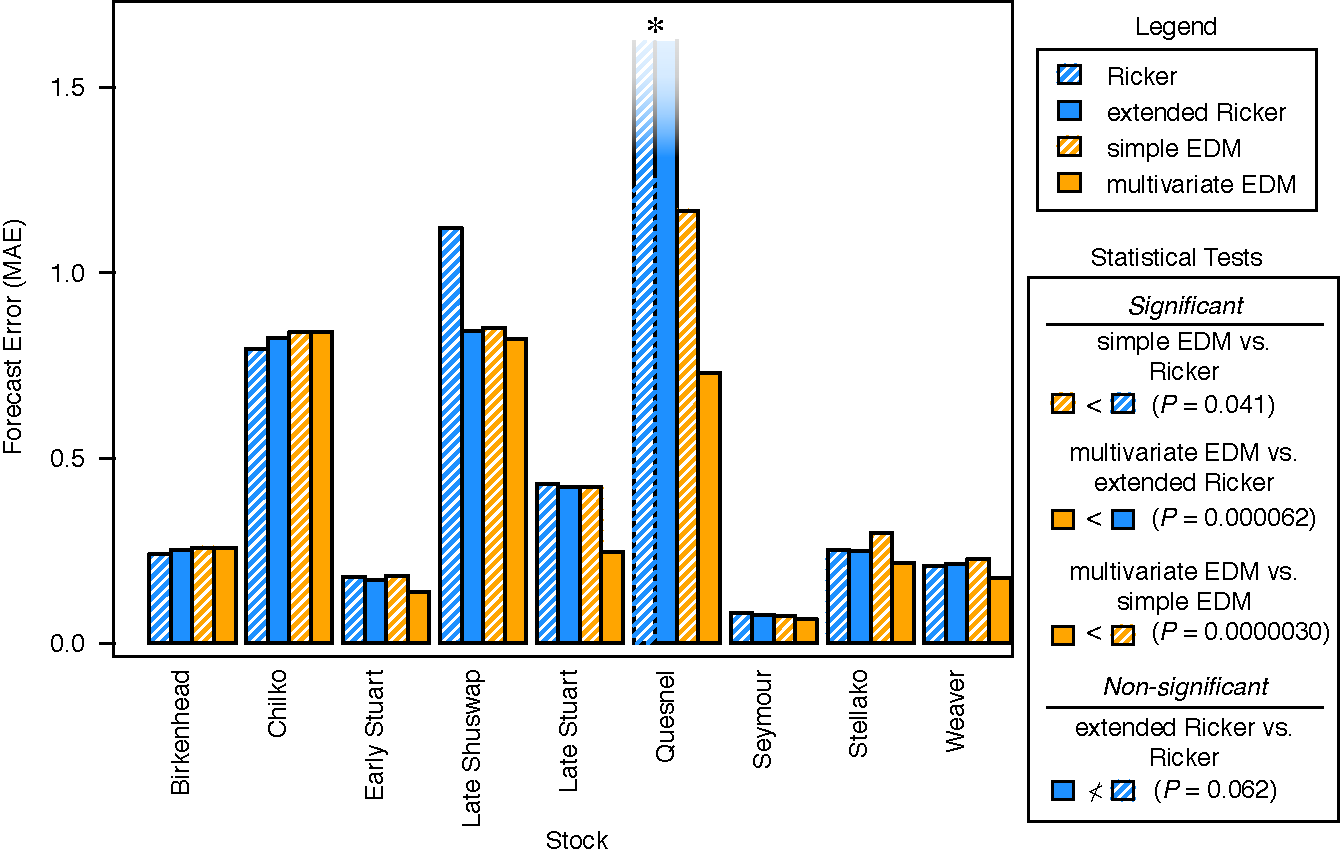
\includegraphics[width=\maxwidth{\textwidth}]{fig_salmon_s3.pdf}\end{center}
\caption[Comparison of forecast precision using MAE.]{\textbf{Comparison of forecast precision using MAE.}\newline
The simple EDM model has lower error than the equivalent Ricker model, [$t_{(493)} = -1.75$, $P = 0.041$]. Including environmental data significantly improves precision for the EDM models [$t_{(493)} = -4.58$, $P = 3.0\times10^{-6}$], but not for the Ricker models [$t_{(493)} = -1.54$, $P = 0.062$], and the resulting multivariate EDM models also have significantly lower error than the Ricker equivalents [$t_{(493)} = -3.87$, $P = 6.2\times10^{-5}$].\newline
\hspace{\linewidth}
* Note that the error for the Ricker and extended Ricker model extends beyond the upper range shown here. MAE is 2.13 for the Ricker model and 2.06 for the extended Ricker model.}
\label{fig_salmon_model_comparison_mae}
\end{figure}

\subsection{Possible Causal Mechanisms for SST, River Discharge, and the PDO}

The tested variables (river discharge, sea-surface temperature, the Pacific Decadal Oscillation) have been thought to influence sockeye salmon recruitment by being indicative of juvenile mortality in the early marine period (i.e., the first year of ocean residence) \cite{Beamish_2004}. For example, river discharge may improve multivariate EDM forecasts because of its effect on food availability, which is believed to play a role in determining this mortality \cite{Beamish_2012}. By affecting estuarine circulation in the Strait of Georgia, freshwater input (from the Fraser River and other riverine sources) can influence ocean productivity \cite{Beamish_1994}; indeed, river discharge, in combination with wind and other factors, has been linked to low oceanic productivity in the Strait of Georgia that may have contributed to poor returns of sockeye salmon in 2009 \cite{Beamish_2012, Thomson_2012}.

Using multivariate EDM, we do find support for river discharge as an informative variable, with the best EDM model for 4 of the 9 stocks containing river discharge as a coordinate (Table \ref{tab_salmon_forecast_skill}). Furthermore, for these 4 stocks (Early Stuart, Late Shuswap, Late Stuart, and Weaver), nearly all of the top-ranking EDM models include river discharge as a coordinate (i.e., Table \ref{tab_salmon_multivariate_full}). However, other than Late Stuart, there are EDM models excluding river discharge that have similar performance, suggesting that for Early Stuart, Late Shuswap, and Weaver, river discharge may be redundant if other observations of the environmental are available. Thus, while river discharge may be an informative variable, it does not appear to be strictly necessary for skillful predictions, except in the case of Late Stuart.

Pine Island SST also appears to be an important variable, and is included in the best multivariate model for 4 of the 9 stocks (Table \ref{tab_salmon_forecast_skill}). With Pine Island lighthouse located at the boundary between Queen Charlotte Strait and Queen Charlotte Sound (Figure \ref{fig_salmon_map}), the measured SST could be informative about the conditions that juvenile sockeye salmon experience after exiting the Strait of Georgia. That Pine Island SST can be informative about recruitment resonates with evidence that anomalous conditions in this area during 2007 were associated with low returns 2 years later (2009), while favorable conditions (low freshwater runoff and moderate northerly winds) in 2008 were associated with record high returns in 2010 \cite{Thomson_2012}. Here, only the Quesnel stock seems to require Pine Island SST for skillful forecasts, as the best model for Quesnel excluding this variable is much less skillful. For the remaining 3 stocks where the best EDM model included Pine Island SST, there were alternative multivariate EDM models including only other variables that showed very similar performance (Table \ref{tab_salmon_multivariate_full}). This suggests that the information in Pine Island SST relevant for predicting recruitment in these stocks may be duplicated in other environmental variables (see discussion in main text on non-uniqueness).

Lastly, although many studies \cite{Mantua_1997, Beamish_1997, Beamish_2004a} have found that decadal-scale climate and oceanic indicators, such as the PDO, are predictive of \emph{regional} productivity for Pacific salmon, one important question is whether this relationship holds at the individual stock level (i.e., do all stocks rise and fall in sync with one another). Among the Fraser River sockeye salmon, at least, there do not appear to be consistent patterns: there has been an overall decline since the early 1990s, but productivity for some stocks (e.g., Early Stuart) has been declining since the 1960s, while others (e.g., Late Shuswap, Weaver) have not exhibited a declining trend at all \cite{Grant_2010}. Our results similarly show no uniform effect of the PDO, as the best EDM model only includes the PDO as a coordinate for 2 of 9 stocks. In both cases (Stellako and Quesnel), however, performance is substantially improved when other variables are included compared to the model that includes just the PDO (Table \ref{tab_salmon_multivariate_full}). Thus, while the PDO may be informative for overall productivity of the Fraser River system, individual stocks appear to be sensitive to more localized environmental conditions; thus including additional (local) environmental variables is essential for improving forecasts for those stocks.

\begin{figure}[!ht]
\begin{center}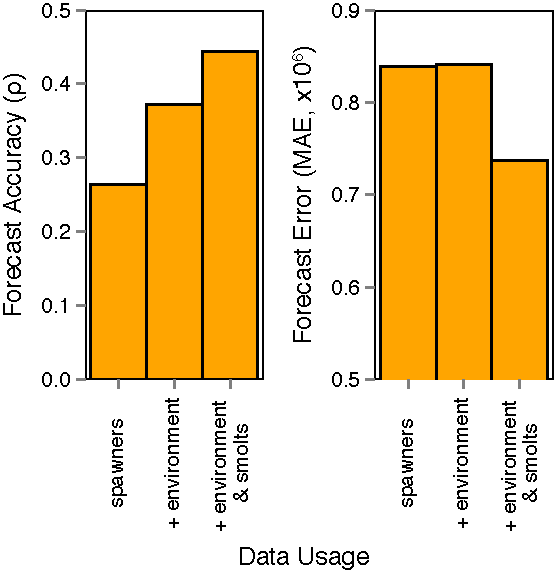
\includegraphics[width=\maxwidth{\textwidth}]{fig_salmon_s4.pdf}\end{center}
\caption[Including smolt data into the Chilko EDM model]{\textbf{Including smolt data into the Chilko EDM model}\newline
For the Chilko stock, adding smolt time series as a coordinate in the best environmental EDM model (spawners \& May Entrance Island SST \& the PDO) improves both accuracy and error.}
\label{fig_salmon_chilko_smolt_model}
\end{figure}

\subsection{Including Smolt Data into EDM Models}

For the Chilko stock, even an exhaustive search for the best possible multivariate EDM model did not produce very accurate forecasts ($\rho < 0.4$, Figure \ref{fig_salmon_chilko_smolt_model}). One possible explanation is that the relationship between spawner abundance and recruits is complex, such that a reconstruction using spawning stock and the tested environmental variables does not uniquely determine recruitment. In such cases, additional observations, such as other environmental factors or measures of salmon abundance at different ages, could resolve singularities in the reconstruction, thereby improving forecasts. For the Chilko stock, a long time series of smolt abundance is available, allowing us to include this variables as an additional coordinate in the multivariate EDM model (Equation \ref{eqn_chilko_smolt}, $J_t^\prime$ is smolt abundance normalized to the current cycle line). Testing this model, we found improvements in both accuracy and error (Figure \ref{fig_salmon_chilko_smolt_model}).

\begin{equation}
\label{eqn_chilko_smolt}
\vec{x}_t = \langle S_t^\prime, J_t^\prime, \mathrm{ET}_{t+2, \mathrm{May}}, \mathrm{PDO}_{t+2}\rangle
\end{equation}

Although the added expense of collecting this kind of data many not be reasonable for all stocks (particularly those that are already very predictable using the tested variables), these observations of sockeye at different ages are additional sources of information that could potentially improve forecasts, giving managers the ability to make trade-offs between data collection and predictability.

\subsection{Estimating Uncertainty for Simplex Projection Forecasts}

We note that the EDM models presented here produce point estimates for the number of returning sockeye salmon. However, fisheries management protocols often require an estimate of the uncertainty surrounding each forecast (i.e., confidence intervals) in order to evaluate the risks associated with management actions. Within the EDM framework, this uncertainty can be addressed in several ways. For example, the relative divergence of nearby trajectories in the reconstructed state space measures how sensitive the future will be to the current state, and is therefore directly indicative of forecast uncertainty. Here we demonstrate a simple implementation of this idea, by noting that the simplex projection method produces forecasts by computing a weighted average of the target variable, $y$ (equation \ref{eqn_simplex_scalar} from the main text):

\begin{equation*}
\hat{y}_{s+h} = \left(\sum_{i=1}^{b}{w_i\left(s\right)y_{n(s, i)+h}}\right) \bigg/ \sum_{i=1}^{b}{w_i\left(s\right)}. \tag{\ref{eqn_simplex_scalar} revisited}
\end{equation*}

In effect, the values of $y_{n(s, i)+h}$ can be thought of as the sample space for the desired prediction, where each value has probability $p_i(s) = \frac{w_i(s)}{\sum_{i=1}^{b}{w_i(s)}}$. Equation \ref{eqn_simplex_scalar} computes a forecast as the expected value of this probability mass function. This idea can then be extended to the second moment of this function in order to compute a variance:

\begin{equation}
\mathrm{Var}\left(\hat{y}_{s+h}\right) = \mathrm{E}\left[\left(y_{n(s, i)+h} - \hat{y}_{s+h}\right)^2\right] = \frac{\sum_{i=1}^{b}{w_i(s)\left(y_{n(s, i)+h} - \hat{y}_{s+h}\right)^2}}{\sum_{i=1}^{b}{w_i\left(s\right)}}
\end{equation}

Note that as the difference between each neighbor's forecast and the weighted average increases, variance will also increase, thus tracking the divergence of the nearest neighbors.

Because simplex projection is used to forecast relative age 4 and age 5 recruits, which are linearly combined to forecast returns (see Materials and Methods), we can similarly compute the variance of returns:

\begin{align}
\begin{split}
\mathrm{Var}\left(\hat{N}_t\right) &= \mathrm{Var}\left(\hat{R}_{4, t-4}\right) + \mathrm{Var}\left(\hat{R}_{5, t-5}\right) + \mathrm{Cov}\left(\hat{R}_{4, t-4}, \hat{R}_{5, t-5}\right)\\
\mathrm{Var}\left(\hat{R}_{a, t}\right) &= \mathrm{Var}\left(\hat{R}_{a, t}^\prime\right) \cdot \left(\sigma_k\left(R_a\right)\right)^2
\end{split}
\end{align}

Here, because the age 4 and age 5 recruits are computed from separate data, we can assume that the covariance is 0 (because the selection of nearest neighbors used to compute $\hat{R}_{4, t-4}$ are independent of those used to compute $\hat{R}_{5, t-5}$).

\begin{figure}[!ht]
\begin{center}\includegraphics[width=\maxwidth{\textwidth}]{fig_salmon_s5.pdf}\end{center}
\caption[Standard errors for EDM forecasts of Late Shuswap returns.]{\textbf{Standard errors for EDM forecasts of Late Shuswap returns.}\newline
Extending the simplex projection algorithm, standard errors for each forecast can be computed. Here, the predictions of the multivariate EDM model are plotted against observations for the Late Shuswap stock.}
\label{fig_salmon_standard_error}
\end{figure}

This is demonstrated in Figure \ref{fig_salmon_standard_error} for the best multivariate EDM model of the Late Shuswap stock. Plotting the EDM forecasts along with standard errors, it is clear that there is good correspondence: variability is higher for the dominant cycle line (as would be expected) and forecasts are generally within 1 standard error of the realized returns.

\section{Acknowledgments}
The authors thank Michael Fogarty, Terry Beacham, Brad Werner, Ethan Deyle, Charles Perretti, and two anonymous reviewers for their feedback on this work. This research is supported by a National Science Foundation Graduate Research Fellowship (HY), National Science Foundation Grant No. DEB-1020372 (GS, HY), Foundation for the Advancement of Outstanding Scholarship and Ministry of Science and Technology of Taiwan (CHH), NSF-NOAA Comparative Analysis of Marine Ecosystem Organization (CAMEO) program Grant NA08OAR\-4320894 / CAMEO (GS), the Sugihara Family Trust (GS), the Deutsche Bank-Jameson Complexity Studies Fund (GS), and the McQuown Chair in Natural Science (GS).

Chapter \ref{chap_salmon_environment}, in full, is a reprint of material published by the National Academies Press as: Hao Ye, Richard J. Beamish, Sarah M. Glaser, Sue C.H. Grant, Chih-hao Hsieh, Laura J. Richards, Jon T. Schnute, and George Sugihara. (2015) Equation-free mechanistic ecosystem forecasting using empirical dynamic modeling. \emph{Proceedings of the National Academy of Sciences} 112: E1569-E1576. The dissertation author was the primary investigator and author of this paper.